\chapter{Iron in Ancient India: Wrought Iron to Steel-From Pins to Pillars}\label{chapter4}

\lhead[\small\thepage\quad chapter IV]{}

We have examined at length the issue of origin of iron in India. In this chapter we propose to evaluate important issues related to iron technology like the process of development of iron technology which involved a proper understanding of behaviour of material under different conditions; smelting and forging techniques; pattern of adaptation of newly developed metal in form of wrought iron; procurement and find spots of suitable ores, ancient mining techniques and the tool typology fashioned at different cultural stages. Our evaluation is based primarily on archaeological evidence. However, India has a rich literary heritage which substantiates and provides fillip to the cultural reconstructions therefore it has been given due importance. Historically speaking, iron took a long time to come of age and prove its merit as a utilitarian metal. The metallurgy of iron had a long gestation period spanning over centuries. This may be viewed as a saga of evolution of metallurgy from simple, crude wrought iron to steely iron which made a niche for itself in the ancient world. 

In most ancient civilizations of the Old World, including India three stages of development of iron metallurgy have been discerned. Snodgrass (1980) while discussing iron in the Mediterranean region classified the developmental stages of iron technology as Stage I, II, and III.  At the earliest level, it has been argued that iron, a distinct metal of great value (four-five times more expensive than gold, as shown in chapter II) does appear on the scene but was more of a status symbol than a metal of common use. Iron at Stage I was primarily ornamental than functional. In several parts of the world one comes across bimetallic objects like gold or bronze daggers with iron blades or some objects that are parts of the ‘dress uniform’ fashioned and used for their {\it costliness} rather than their {\it effectiveness}. Generally, such artefacts are of wrought iron or at the most carburised (possibly due to forging technique adopted during the early stages). Several of the early specimens of iron found in Egypt, Mesopotamia or in the neighbouring West Asian countries like Iran are meteoritic in nature and were used to enhance the beauty and value of gold or ceremonial bronze objects. The Bronze Age chieftains donned such iron ‘weapons’ as status symbols. In India, so far we have rarely come across iron objects of this type. Only bits of iron have been found at some sites in pre-iron stage, such as at Noh in Rajasthan (in BRW phase). At the earliest stage of its occurrence, small pins, rods, nails or arrowheads of wrought iron were fashioned. A few pieces of bimetallic objects of iron and bronze have come to light from Andhra and Vidarbh megalithic burials (personal observation). Iron at this stage had hardly an edge over the earlier metal (copper-bronze) tools in use. Occasional carburisation has been detected on analysis of artefacts of this period.

At stage II, the Middle Iron Age in Old World civilizations, though objects of functional utility are present, their number is ‘less than bronze for implements of practical use’. In India iron does not fully replace bronze even for hunting or war objects till much later. Sites like Hastinapur (PGW phase, {\it  c}. 1000 BCE) have yielded copper arrowheads. Iron implements at this stage (our Early Iron) were sometimes replicas of early bone or stone objects of Neolithic-Chalcolithic period indicating a gradual transformation of medium that is modelled after bone prototypes such as a 700-600 BCE socketed arrowhead with holes for fastening from Khairadih (see Tripathi 2018, Pl.XIII.20; Fig.~27.20).~Deliberate carburisation has been noted in certain cases from this period onwards. Textual evidence, such as from the early Buddhist literature also corroborates knowledge of carburization, as will be discussed below. 

At stage III, Snodgrass (op.cit) states “iron predominates over bronze as the working metal, although it need not, and usually does not, completely displace bronze even in this role”. However, the metallurgy of iron improved tremendously during this phase of development. It is at this stage of technological development that Alexander was gifted with steel ingots after his victorious expedition in the North-western parts of India in $4^{\rm th}$ century BCE. Ktesias ($5^{\rm th}$ - $4^{\rm th}$ BCE) mentioned about high quality iron swords of Indian origin that were presented to him in Persian court by the King and his mother.~Sushruta ($6^{\rm th}$–$5^{\rm th}$ century BCE) had evolved surgical methods of treatment and had commissioned steel instruments for performing surgery. A good number of surgical instruments have been mentioned in {\it Sushruta Samhita}. Our recent analyses of iron objects at Rutherford Appleton Lab (Oxford) further confirmed this assumption. As mentioned above, a close analysis revealed an object from the site of Latif Shah we identified as surgical knife (Fig.~7.~A and Fig.~7.~B). Its tip was covered with a thin copper- sheet, presumably for some special function in surgery. 

These well documented instances prove beyond doubt that high quality iron was being produced in India at least by the $5^{\rm th} - 4^{\rm th}$ century BCE or even earlier. At Iron III or Late Iron stage, a rich variety of tools, implements, weapons, household objects become common-place (see tables of objects of iron). The 7375 mm long, 416mm in diameter (at bottom) and 304 mm at top Mehrauli iron pillar weighing 6096 kg belongs to the Gupta period ($4^{\rm th}-5^{\rm th}$ century CE; Fig.~28~a,~b; discussed below in detail) an age of culmination of technological skill. Sophisticated weapons like tridents, swords, and caltrops reportedly of good quality steel were used. This brief narration of occurrence of iron objects from different contexts makes a detailed examination of metallurgical developments inevitable at this juncture.

\vspace{-.3cm}

\section*{Development of Metallurgy\hfill \break in Ancient India}\label{section-1}

An overview of the iron metallurgy over the centuries clearly reveals distinct metallurgical developments and process of adaptation of tools and implements being produced. On the basis of status of metallurgy, and the nature of artefacts being produced at different stages, I propose to classify these stages as: the ‘Age of Commencement’, ‘Age of Consolidation’ and ‘Age of Culmination’ of iron metallurgy as detailed below: 
\begin{enumerate}
\item The Age of Commencement- Early Iron Age- from the beginning to $7^{\rm th} -6^{\rm th}$ century BCE
\item The Age of Consolidation- Middle Iron Age – $7^{\rm th} – 6^{\rm th}$ BCE to $2^{\rm nd}$ -$1^{\rm st}$ century BCE
\item The Age of Culmination- Late Iron Age- $2^{\rm nd} -1^{\rm st}$ century BCE to the historical period
\end{enumerate}

\vspace{-.5cm}

\subsection*{1.i. The Age of Commencement- Early Iron Age (From the beginning (18/1700 BCE to $7^{\rm th} -6^{\rm th}$ century BCE)}\label{chapter4-subsection-1}

At most of the ancient sites iron appears for the first time between the $2^{\rm nd}$ millennium BCE and beginning of the $1^{\rm st}$ millennium BCE. It comes to be used around this time in several parts of the country. There appears to be a qualitative and quantitative improvement in iron technology even within this stage. At the earliest stage there appear some bits and pieces at sites like Noh, District Bharatpur in Rajasthan (with pre- PGW, Black-and-Red ware cultural strata datable to c.~1300-1200 BCE). In the very next phase hunting tools like arrowheads, spearheads, nails etc. appear. We come across only a few iron objects at Early Iron Age (see Table~\ref{table IV.8}). Before the regular beginning of iron, shapeless tiny bits of iron were noted at Noh in Pre-PGW period. Hulas yielded only slag pieces. Bahiri has unique evidence: heaps of slag but no finished iron objects at all (an early smelting centre?). The site of Noh thus manifests evolutionary stages in iron metallurgy. Within a short span of time the stray occurrence of bits of iron seen at these places were followed by finished objects of iron but in small numbers. At most of the sites of Early Iron Age phase at PGW Period at sites like Noh and Jodhpura in Rajasthan; Malhar, Raja Nal-Ka-Tila, Koldihwa, Raipura and Latifshah in the iron ore rich zone of the Vindhyas and Jhusi, Kausambi, Aktha (Varanasi) Lahuradeva (belonging to Black-and-Red Ware phase) in the plains iron occurs in early context. These sites have yielded early dates of use of iron dating back to first half of second millennium BCE. Other noteworthy sites of this stage are Ahar in Rajasthan, Prakash, Bahal in Decean and Eran, Kaytha in M.P., Chirand in Bihar, Kausambi, Rajghat in Uttar Pradesh, Hathigra, Mangalkot, Mahisdal, Pandurajar Dhibi in Bengal, Naikund, Takalghat-Khapa, Mahurjhari, Hallur, Kumaranhalli, Tadkanhalli etc. in Vidarbh and peninsular India. 


Koldihwa (I.A.R.$^{1}$ 1973-74: 27), otherwise defined as a Chalcolithic site in the Vindhyan plateau yields an iron axe, arrowheads, crucibles and slag from strata immediately following the Chalcolithic culture. It may be noted here that iron is found along with microliths at many sites in the Vindhyas (in District Mirzapur-Sonbhadra), such as at Morahana Pahar, Baghair Khor, near Bhaisaur and several other so called microlithic sites. Microlithic tools are generally associated with Mesolithic Age. Iron tools found along with microliths may indicate either a continuation of microliths till late or an early beginning of iron in this iron ore-rich belt. Recently, the Vindhya-Kaimur hilly belt has yielded the earliest evidence of iron so far from the site of Malhar and subsequently from Raipura. This evidence is also corroborated by excavations at Raja-Nal-Ka-Tila, not far from the above two sites (Tables,~\ref{table III.1}-~\ref{table III.3} and \ref{table III.9}, \ref{table III.10}). There are consistent radiocarbon dates ranging from 18/17000-1500 BCE to 1100-1000 BCE from these sites (Tewari, 1998, 2003; Tripathi, 2014). These sites yielded iron along with ceramics like BRW and BSW of an early variety. In the considered opinion of the excavators that the dates of beginning of iron at Malhar should go back to pre-1500-1400 BCE (see Table~\ref{table III.2}). The dates from middle of iron bearing strata are: $1200\pm 90$ BCE, $1200\pm100$ BCE, $1423-1307$ Cal. BCE (Birbal Sahni Institute of Palaeobotany, and $1030\pm 90$ (P.R.L.), the calibrated date is for the mid-phase of iron bearing level. Therefore, the dates of beginning of iron at the site should be much earlier. The site of Raipura in Sonbhadra District is also located in the same ore-rich area as Raja Nal- ka -Tila and Malhar. The dominant pottery at the site is Black Slipped Ware, instead of BRW which occurs in larger amounts at many other sites. Iron occurs from Period II onwards at Raipura. Significantly enough, the excavations at Raipura yielded a fairly well preserved furnace with a tuyere-hole (Fig.~\ref{chapter-4-fig8}). Remains of forge have also been found nearby from period III. Stone slabs used for weighing down the bellows have been recovered in situ (Fig.~\ref{chapter-4-fig9}). More interesting is occurrence of an ingot in Period III affirming the local iron production in this workshop-like area (Fig.~\ref{chapter-4-fig10}). The ${}^{14}$C dates from Period II– pre-NBPW period – range from 1800/1700 to 1400/1300 BCE.

\begin{figure}[H]
%~ \renewcommand{\thefigure}{7B}
\setcounter{figure}{7}
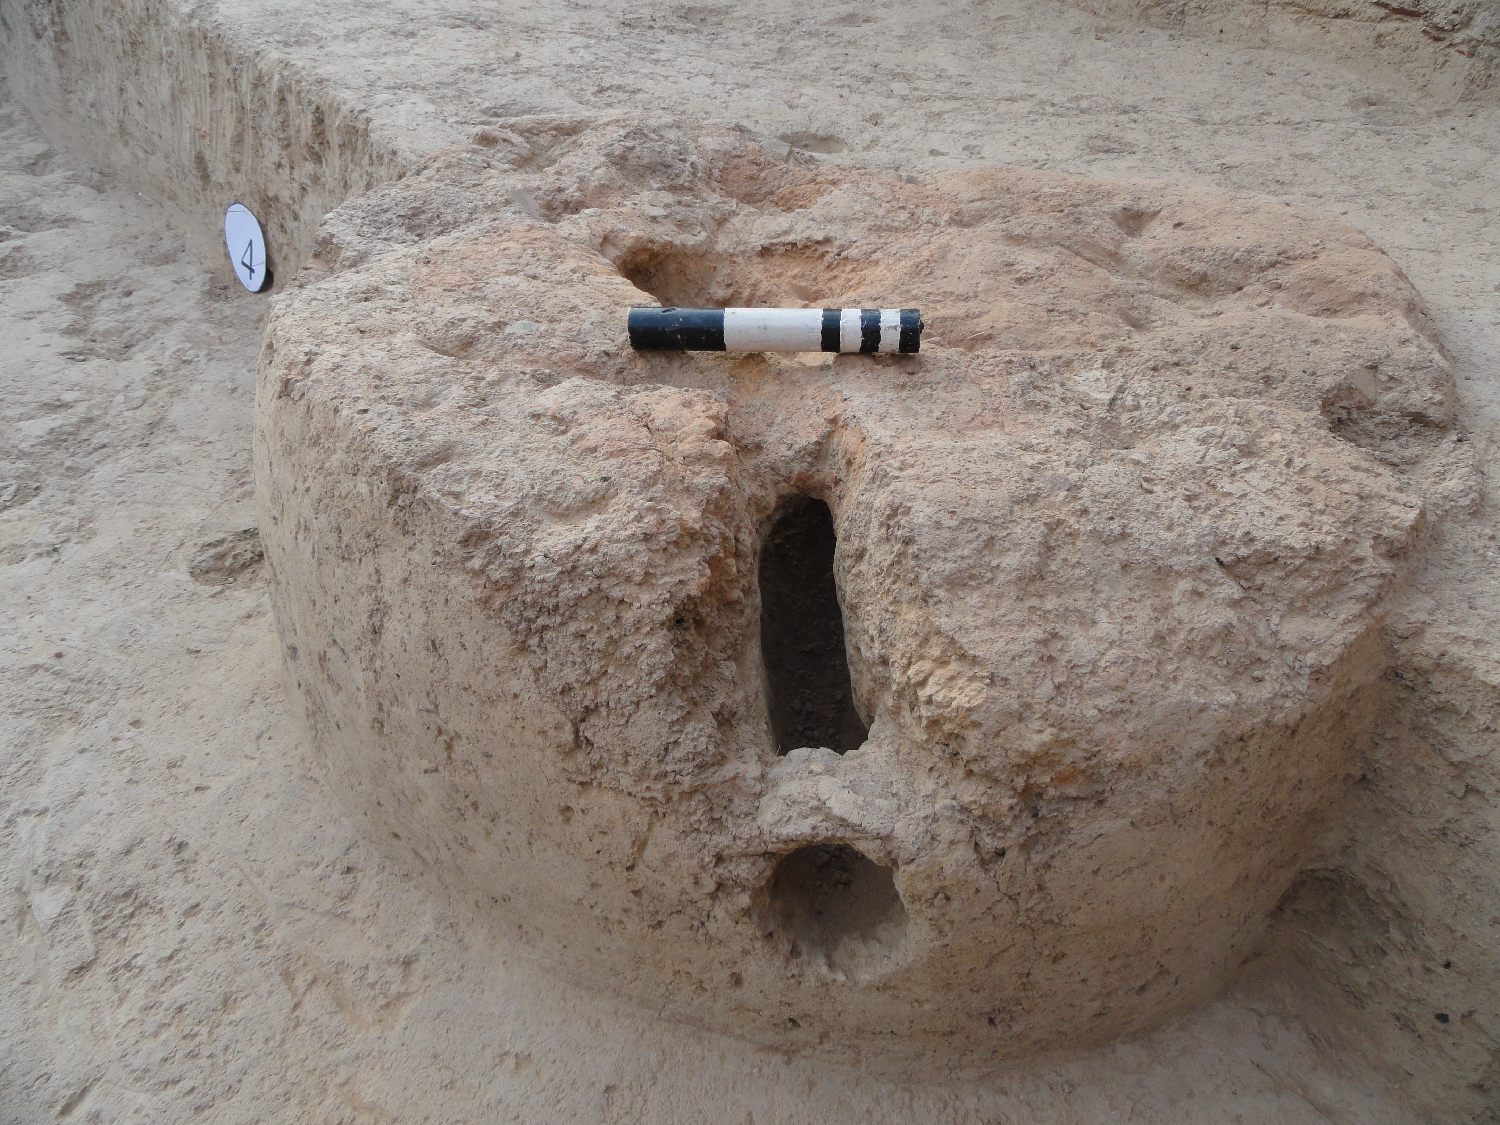
\includegraphics[scale=0.75]{images/chapter-4/fig008.jpg}
\caption{RPA Pd II Pre NBPW}\label{chapter-4-fig8}
\end{figure}

\begin{figure}[H]
%~ \renewcommand{\thefigure}{7B}
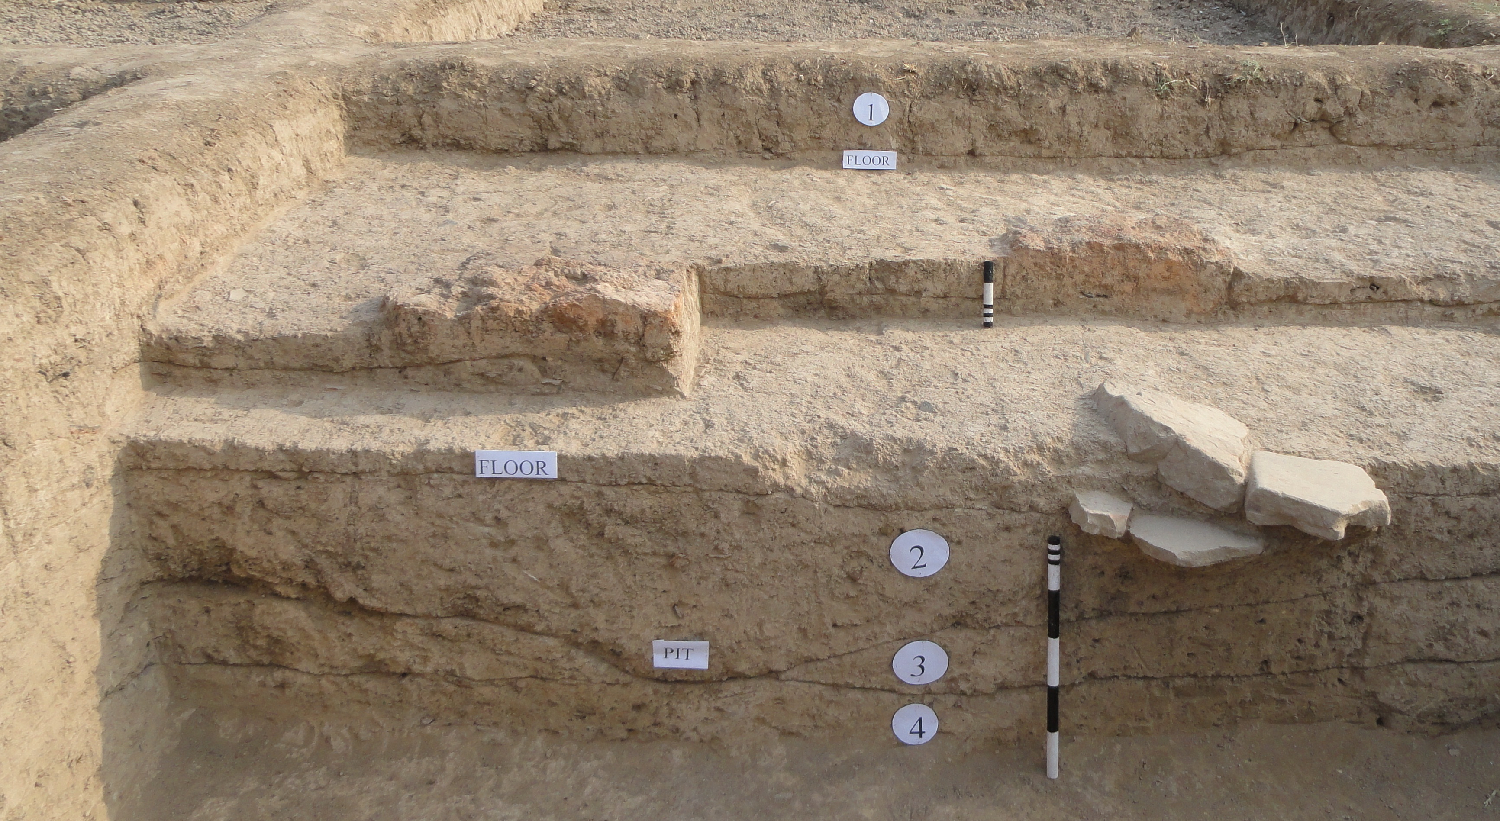
\includegraphics[scale=0.75]{images/chapter-4/fig009.jpg}
\caption{Iron Furnace-Forge Raipura Pd. III}\label{chapter-4-fig9}
\end{figure}

\newpage

\begin{figure}[H]
%~ \renewcommand{\thefigure}{7B}
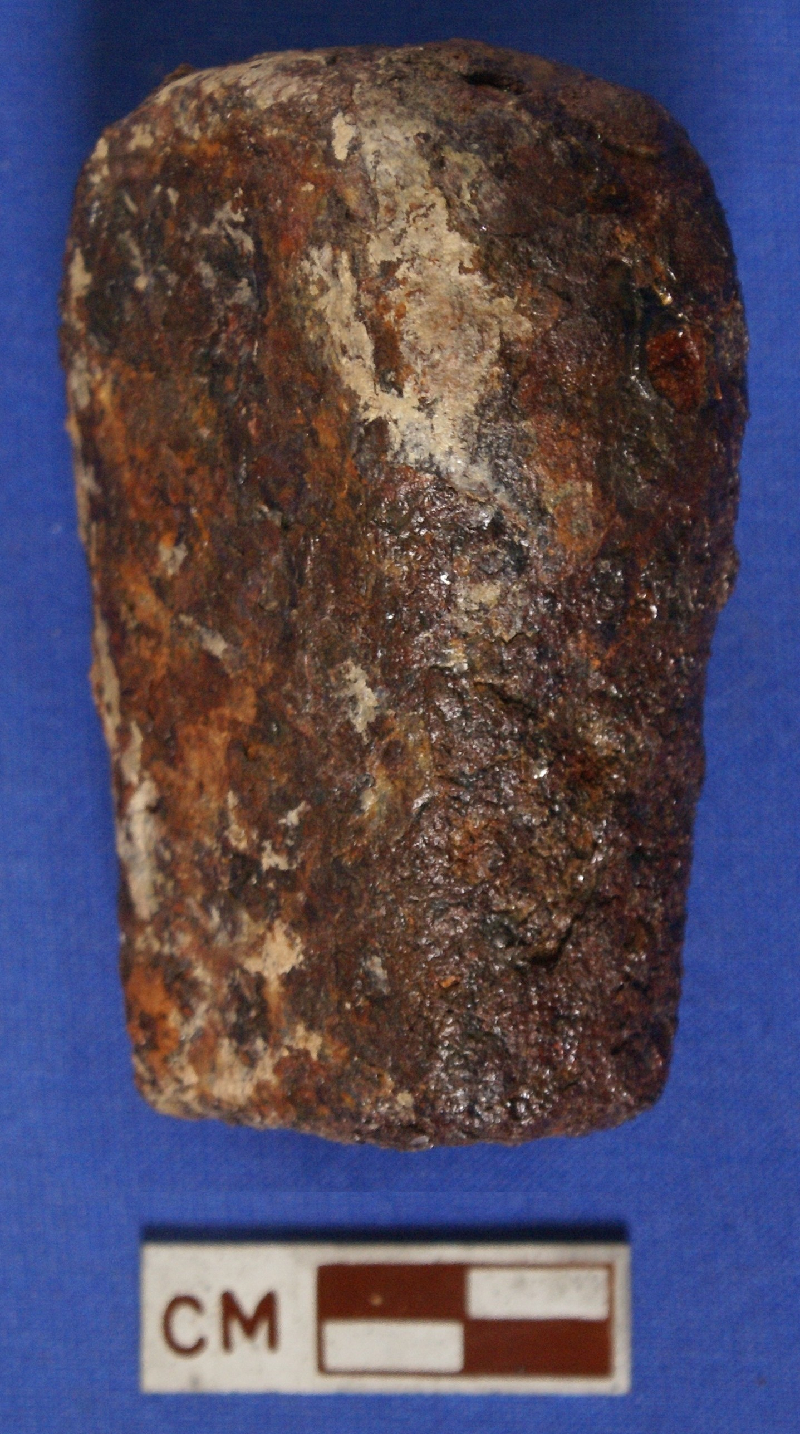
\includegraphics[scale=0.8]{images/chapter-4/fig010.jpg}
\caption{Iron Ingot RPA Pd.III NBPW}\label{chapter-4-fig10}
\end{figure}

%~ Koldihwa (Indian Archaeology - A Review (I.A.R.) 1973-74: 27()), otherwise defined as a Chalcolithic site in the Vindhyan plateau yields an iron axe, arrowheads, crucibles and slag from strata immediately following the Chalcolithic culture. It may be noted here that iron is found along with microliths at many sites in the Vindhyas (in District Mirzapur-Sonbhadra), such as at Morahana Pahar, Baghair Khor, near Bhaisaur and several other so called microlithic sites. Microlithic tools are generally associated with Mesolithic Age. Iron tools found along with microliths may indicate either a continuation of microliths till late or an early beginning of iron in this iron ore-rich belt. Recently, the Vindhya-Kaimur hilly belt has yielded the earliest evidence of iron so far from the site of Malhar and subsequently from Raipura. This evidence is also corroborated by excavations at Raja-Nal-Ka-Tila, not far from the above two sites (Tables,~\ref{table III.1}-~\ref{table III.3} and \ref{table III.9}, \ref{table III.10}). There are consistent radiocarbon dates ranging from 18/17000-1500 BCE to 1100-1000 BCE from these sites (Tewari, 1998, 2003; Tripathi, 2014). These sites yielded iron along with ceramics like BRW and BSW of an early variety. In the considered opinion of the excavators the dates of beginning of iron at Malhar should go back to pre-1500-1400 BCE (see Table~\ref{table III.2}). The dates from middle of iron bearing strata are: $1200\pm 90$ BCE, $1200\pm100$ BCE, $1423-1307$ Cal. BCE (Birbal Sahni Institute of Palaeobotany, and $1030\pm 90$ (P.R.L.), the calibrated date is for the mid-phase of iron bearing level. Therefore, the dates of beginning of iron at the site should be much earlier. The site of Raipura in Sonbhadra District is also located in the same ore-rich area as Raja Nal- ka -Tila and Malhar. The dominant pottery at the site is Black Slipped Ware, instead of BRW which occurs in larger amounts at many other sites. Iron occurs from Period II onwards at Raipura. Significantly enough, the excavations at Raipura yielded a fairly well preserved furnace with a tuyere-hole (Fig.~8). Remains of forge have also been found nearby from period III. Stone slabs used for weighing down the bellows have been recovered in situ (Fig.~9). More interesting is occurrence of an ingot in Period III affirming the local iron production in this workshop-like area (Fig.~10). The ${}^{14}$C dates from Period II– pre-NBPW period – range from 1800/1700 to 1400/1300 BCE.

\vspace{-.3cm}

Chronology of Raipura is discussed in somewhat detail here to reiterate the early incidence of iron production in these parts located in the central part of India. We could pick up charcoal sample from a pit sealed by layer (4), close to the furnace. It has yielded ${}^{14}$C date (BS \# 3536) $1720 \pm 220$ cal BC. There is a deposit of about 20-25 cm underneath this layer. The charcoal sample (PRL 3317) collected from the earliest layer pertaining to Period II from trench ZB-10 yielded a date of $3480\pm110$ BP or 1867 cal BC -1848 cal BC -1774 cal BC-1527 cal BC (1 sigma) or 1932 – 1438 cal BC (2 sigma), see Tables. The dates from two independent agencies, i.e. PRL and Birbal Sahni Institute of Palaeobotany are virtually the same (Tables~\ref{table III.9},~\ref{table III.10}). There is a deposit of about 10-25 cm underneath these layers. Therefore, it may have a still higher antiquity. The region seems to be an iron production centre. Occurrence of an ingot from Period III further supports this contention. Raipura has yielded iron objects as well as furnaces datable from BCE 1700/1600 to 200 that is from its Periods II and III (Pre-NBPW Period and NBPW period, respectively (for details see, Tripathi and Upadhyay, 2013: 149-157). The sites in the Vindhya-Kaimur region– Malhar, Raipura Nal ka Tila and Latifshah with smelting activity – seem to be resource zone for settlements in the plains. The emerging city sites in the Ganga Plain required supply of iron tools and implements, a need which was fulfilled by the above mentioned sites located in the bordering hilly terrain. A symbiotic relationship seemed to have been developed over the centuries between the two eco-zones. 

The sites in the plains which may be termed as consumer area for tools manufactured in the hills bordering the plains, we come across interesting pattern of use of iron artefacts. We propose to deal with the evidence in some detail here. Atranjikhera in district Etah has yielded Painted Gray Ware (henceforth PGW) in a thick deposit of up to 2.50m. The period has been divided into three sub-phases by the excavator (Gaur 1983). The earliest phase has yielded only seven objects and a lump and does not contain even the most elementary types like arrowheads and spearheads. These hunting tools appear in the mid-PGW phase, which has a total of 46 objects. The upper phase has yielded 81 objects thus indicating a rising level of adaptation of iron over a period of 600 years, from 1100/1000 BCE to 600 BCE, the assigned date of PGW culture. This indeed suggests an evolution in use of iron within this period. Jakhera, another site not far from there, yielded an iron ploughshare along with slag and blooms from the earlier phase designated as the proto-PGW phase. Iron appears in the succeeding period from the very beginning of PGW yielding hoe, sickle, spearhead, arrowhead dagger, chopper, chisel, axe, nails, rods etc. (Sahi 1994). At Hastinapur and Alamgirpur in Meerut district iron came in use with PGW. Hastinapur, yielded four objects and some slag. Alamgirpur (with 137 cm. thick deposit) yielded iron right from the earliest levels - a spearhead, a barbed arrowhead, nail and pins being the main objects. Kausambi has yielded a few objects in the BRW phase that should be contemporaneous with Jhusi. The latter has recently been dated by $14^{\rm C}$ to 1107-844 BCE. Recent evidence from Malhar, Raipura and Latif Shah are noteworthy. Iron working workshops complete with furnaces, forges and finished objects in good numbers have been found in an early context (Figs.~ \ref{chapter-4-fig8}-\ref{chapter-4-fig16C}).

\begin{figure}[H]
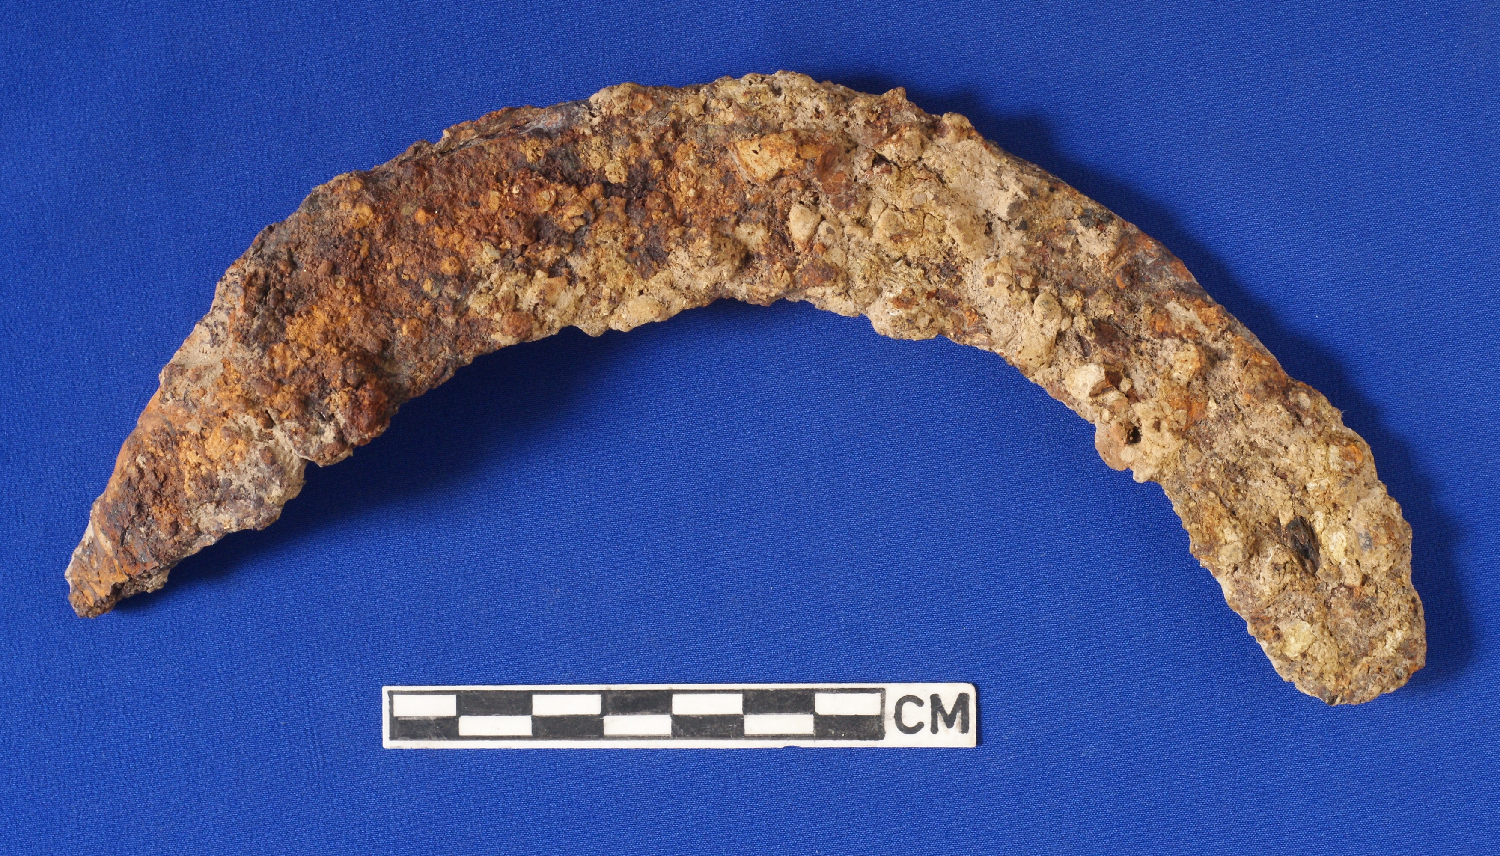
\includegraphics[scale=0.75]{images/chapter-4/fig011.jpg}
\caption{LTS Pd. I BSW Period Bharati 41}\label{chapter-4-fig11}
\end{figure}

\begin{figure}[H]
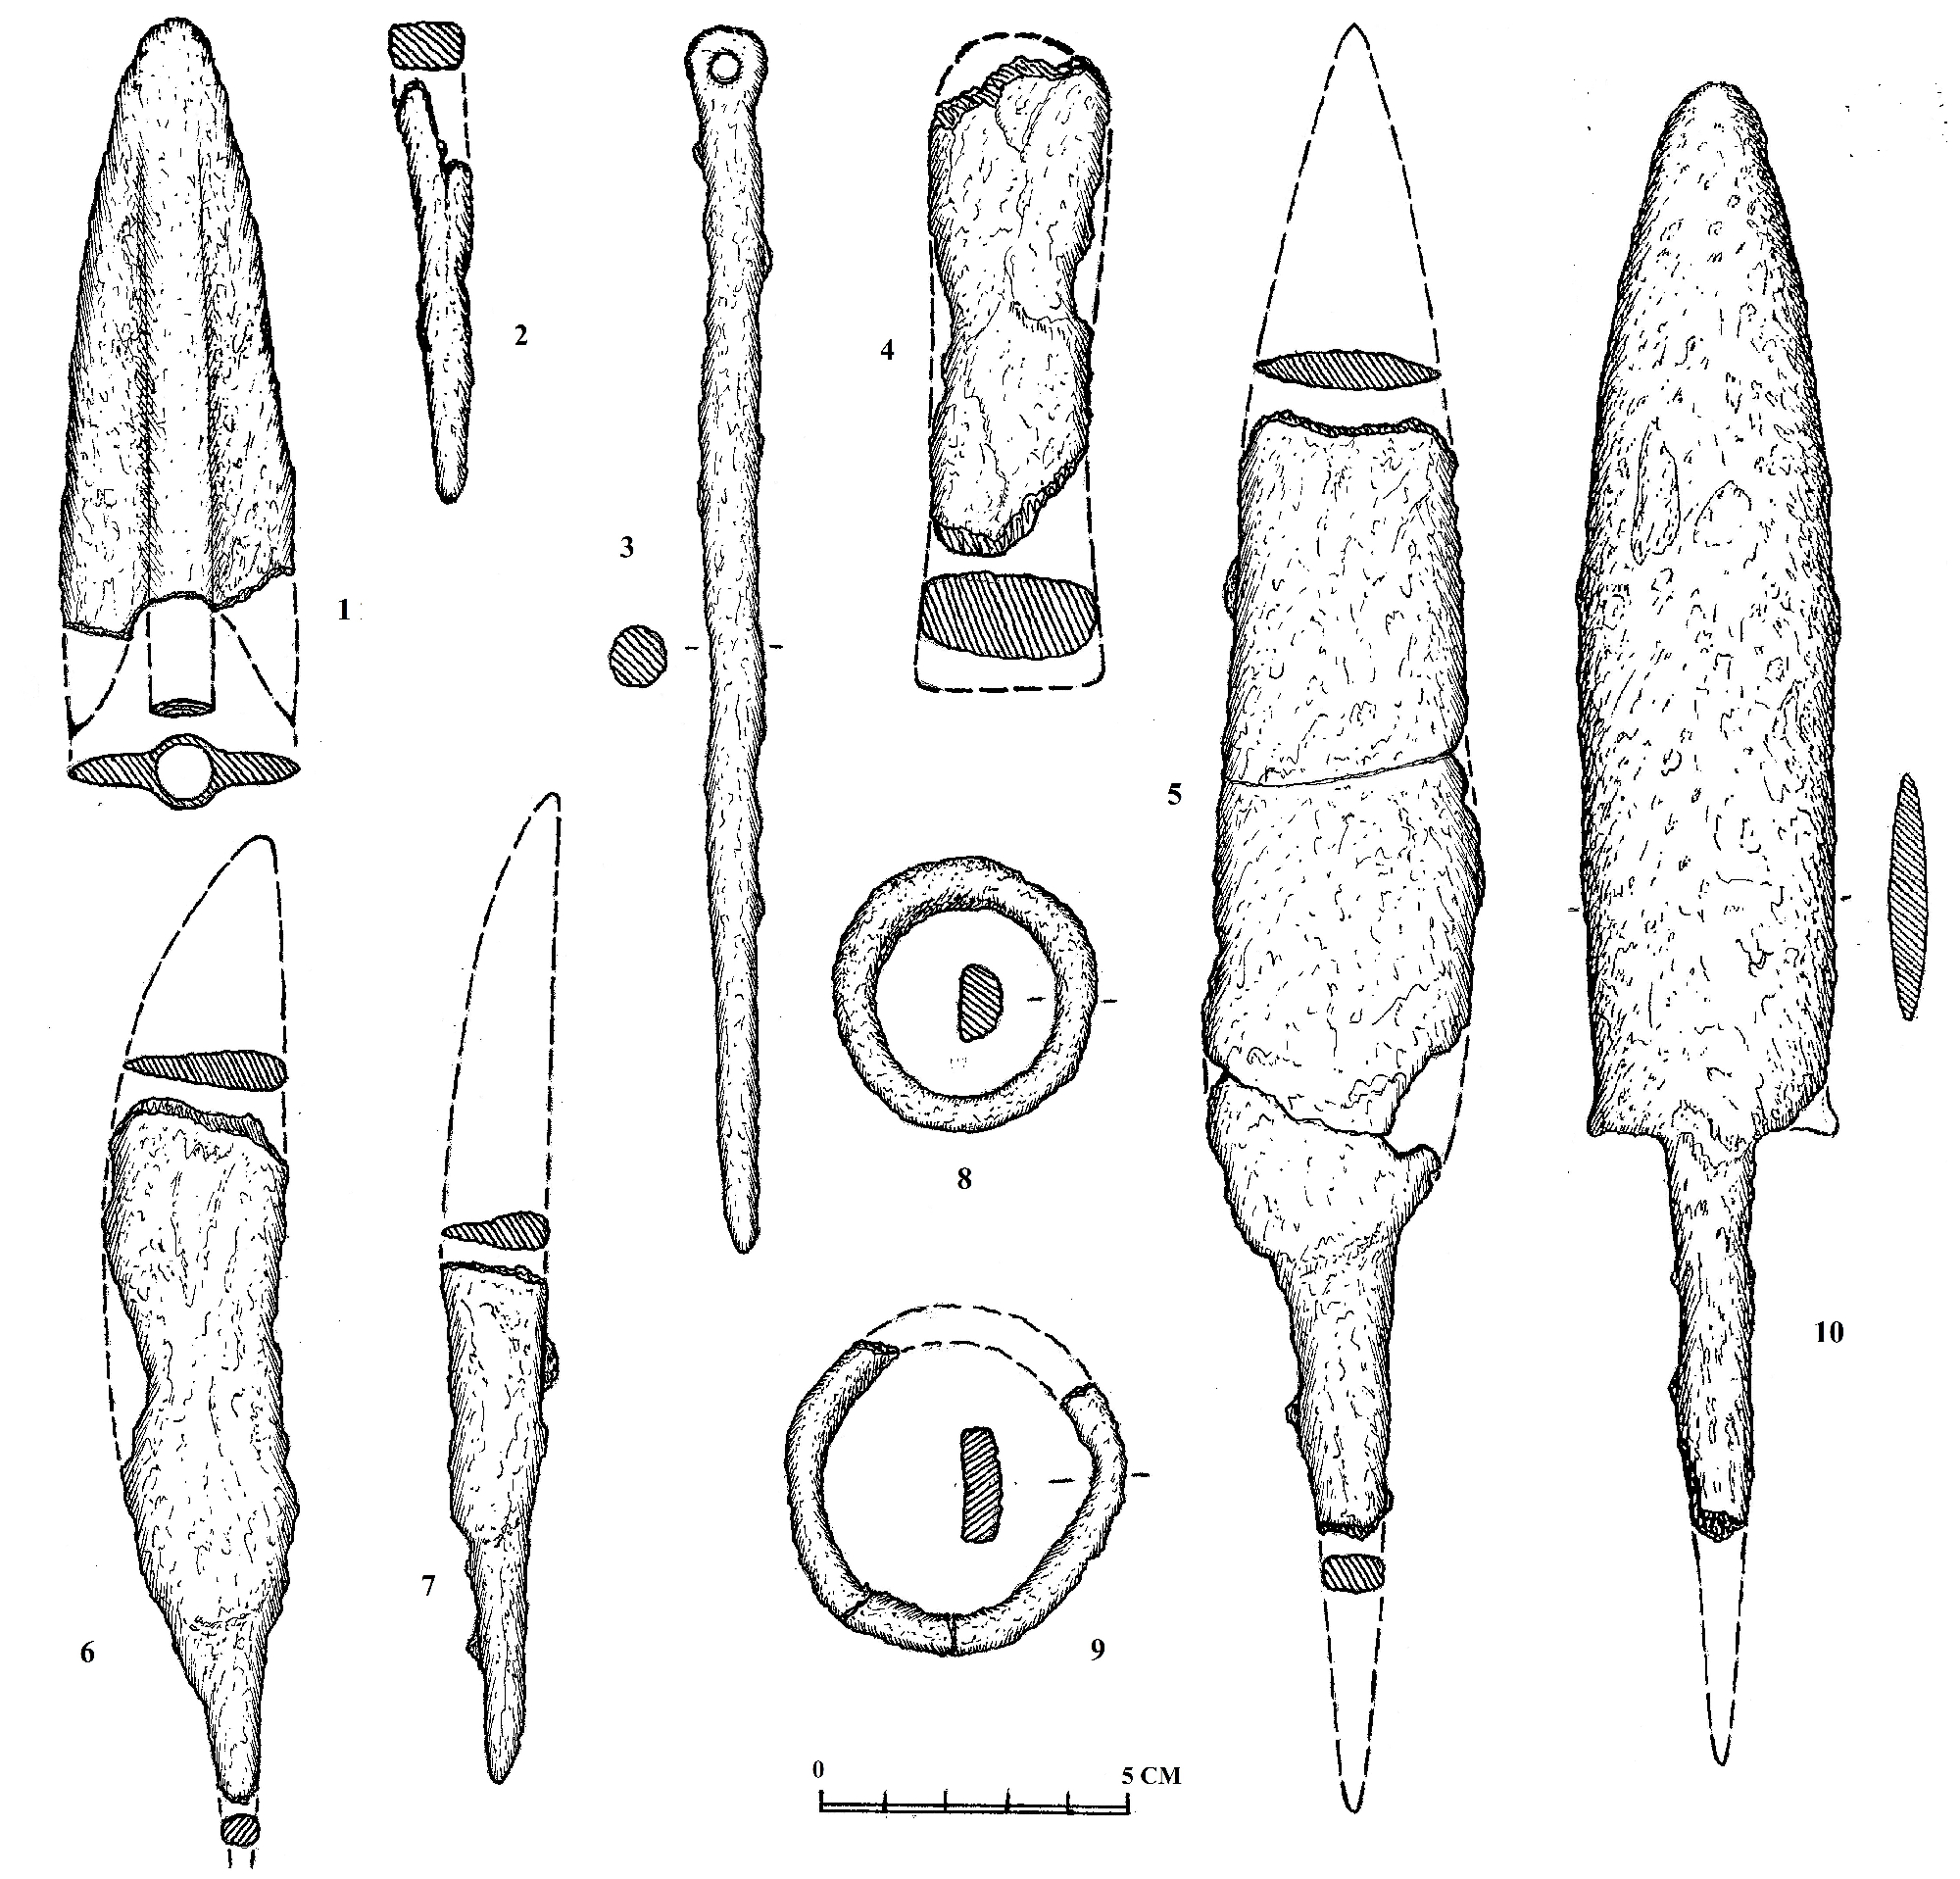
\includegraphics[scale=0.55]{images/chapter-4/fig012.jpg}
\caption{LTS Iron 2016 Pl 4 Pd. I}\label{chapter-4-fig12}
\end{figure}

\begin{figure}[H]
\renewcommand{\thefigure}{13A}
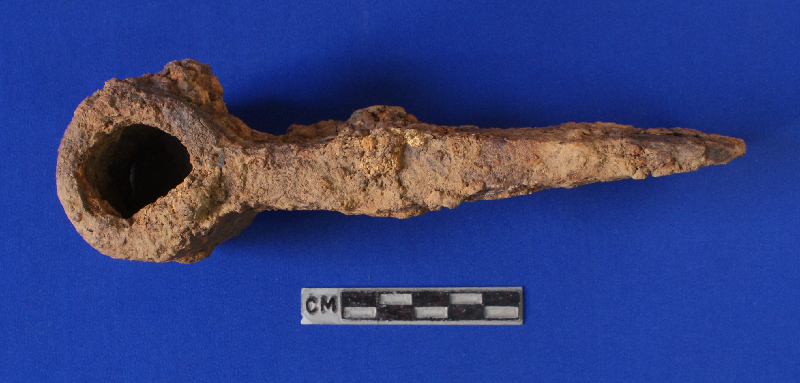
\includegraphics[scale=1.4]{images/chapter-4/fig013A.jpg}
\caption{LTS Pd. II Mid -NBPW phase Bharati 41 p158}\label{chapter-4-fig13A}
\end{figure}

\begin{figure}[H]
\renewcommand{\thefigure}{13B}
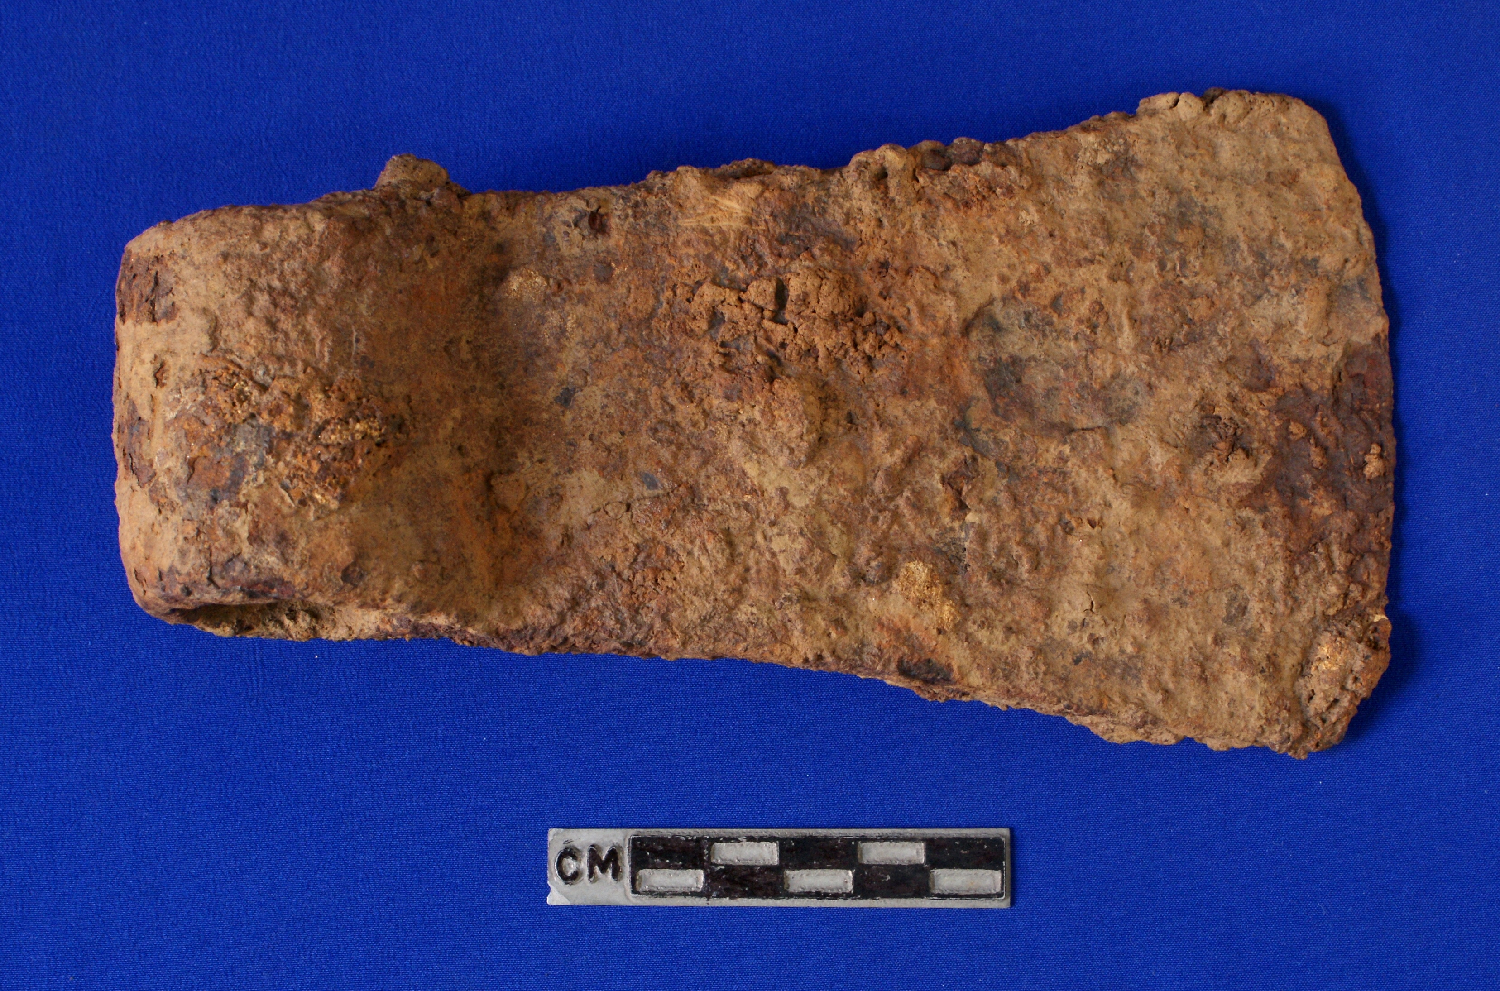
\includegraphics[scale=0.75]{images/chapter-4/fig013B.jpg}
\caption{LTS c. 500 BC Period II, NBPW. Bharati 41 p158}\label{chapter-4-fig13B}
\end{figure}

\newpage

\begin{figure}[H]
\setcounter{figure}{13}
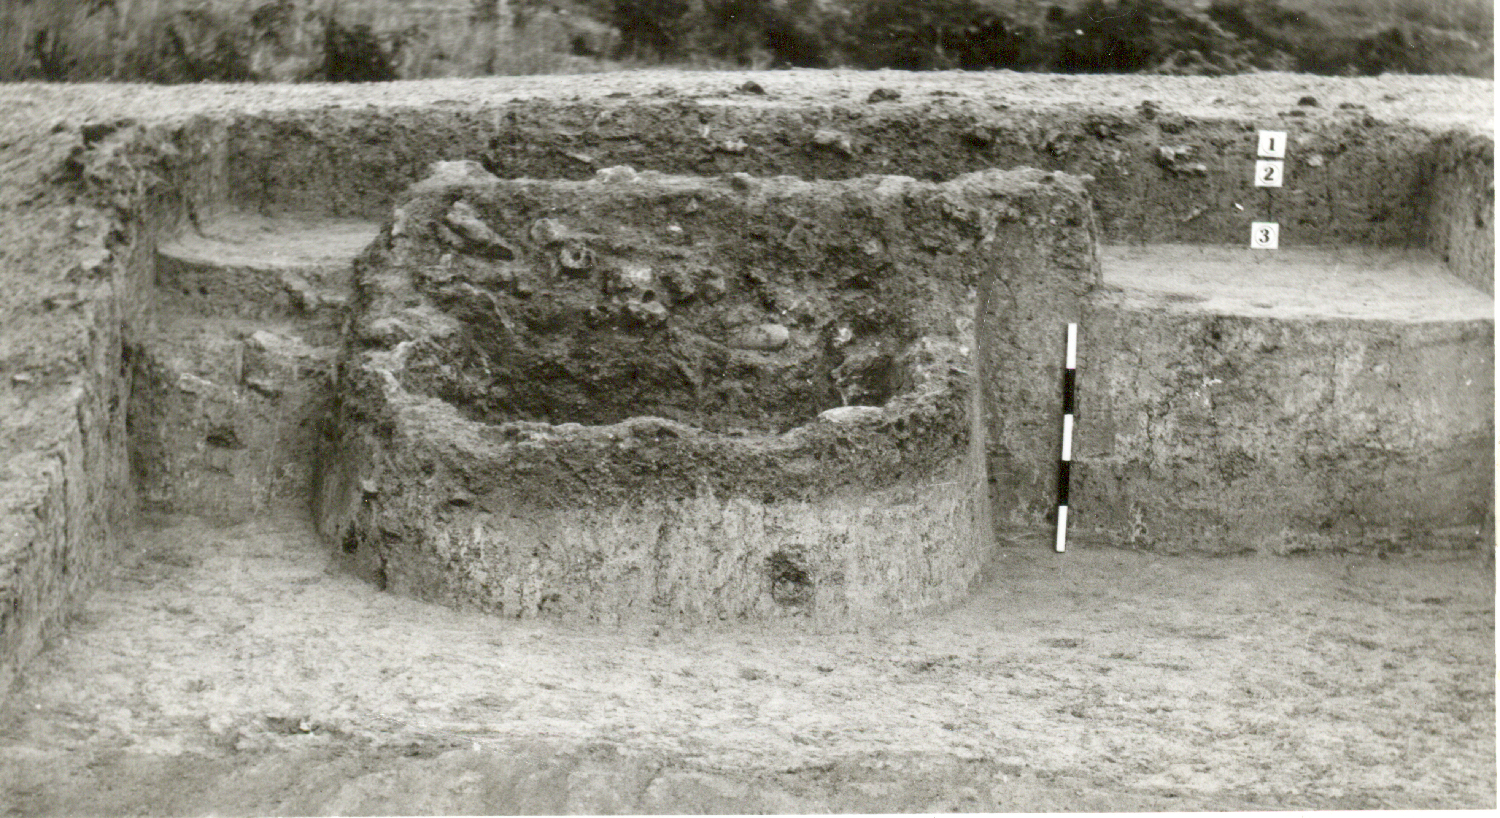
\includegraphics[scale=0.75]{images/chapter-4/fig014.jpg}
\caption{Malhar}\label{chapter-4-fig14}
\end{figure}

\vspace{-.5cm}

A somewhat similar situation is discernible at the site of Mangalkot in West Bengal, (Dutta 1992) in an otherwise Chalcolithic culture with Black-and-Red ware. Unfortunately, such phase-wise detailed data on occurrence of metal objects are not forthcoming from most of the other sites. But even in the absence of such statistical data, a pattern of evolution may be discerned from the E.I.A. (Early Iron Age) sites. Mangalkot has yielded 8 finished (arrowhead, spearhead, nail and rod) and 8 unidentifiable pieces of iron objects from the earliest phases of Chalcolithic culture from a small trench of 6 x 6 m. A furnace has also been reported from the lowest level dated to 1200 BCE. The succeeding period has yielded newer shapes like sickle, chisel, peg, knife, rod etc. Pandurajar Dhibi has also yielded finished iron objects like arrowheads and a knife (or sickle?) blade from mid phase of Chalcolithic culture that is contemporaneous with the above period.

The south Indian megalithic burials are quite rich in iron (in our zones E and F). As mentioned earlier, swords, spikes, tridents, horse bits and also utensils of iron are recovered along with usual objects generally associated with this period, i.e. arrowheads, spearheads, chisels, axes, fish hooks and bangles (Table~\ref{table IV.11}).

It may be noted here that the metallurgical skill was still evolving during this phase. The wrought iron objects had plenty of slag inclusions in the matrix of ferrite indicating a solid-state reduction (Fig.~17 C, D, Tadkanhalli). The iron samples analysed from the site of Hatigra dated 1100-1000 BCE. (Ghosh and Chattopadhyay 1987-88) had observed a widmannstatten structure due to prolonged exposure at a temperature of about $1200 {}^{\circ}C$ followed by a slow cooling (Fig.~18. A, B, C). It is ‘low carbon hypoeutectic steel’. Bhanu Prakash (personal communication) has thought it to be hypereutectoid $Fe C > 0.8\%$ steel. The concen\-tration of carbon visible on the edges in the metallograph indicates carburisation.~The furnaces at this stage could hardly generate sufficiently high temperature. The analysed slag specimens from Hatigra and Pandurajar Dhibi (Chattopadhyay, 2004, 102) and from Mangalkot (Dutta op. cit., 303, Fig.~19 A, B, and C}) have a high percentage of silica in them (22.48- 29.26 \% at Mangalkot). Other impurities reported are traces of nickel, cobalt and copper. The analysis indicates the nature of ore used and at the same time inefficient smelting by the early Chalcolithic smelters (who must have been basically adept in copper working).  Remnants of a furnace are found. But they are broken and do not give much idea of the shape of the furnace. Iron from Tadkanhalli (dated by T.L. to $13^{\rm th}$ -$14^{\rm th}$ BCE) has been analysed by N.R.L.C., Lucknow (Fig.~17 C and D op.cit). The micrograph shows slag inclusion, although it has been reported to indicate pearlite in the structure suggesting it to be a steely iron. However, this has been contested by Prakash on technical grounds (personal communication). So far, the samples analysed from E.I.A. indicate a solid-state reduction at a low temperature in elementary furnaces. But samples analysed from the megalithic site of Mahurjhari in Maharashtra in Deccan as noted earlier, shows evidence of steeling (Deshpande 2010: 636-639). This analysis clearly indicates tempering and quenching of artefacts by megalithic iron workers of the Deccan as early as 900 BCE. Whether this was incidental or deliberate cannot be ascertained in view of limited study of this nature. However, such evidence has not been reported from other Early Iron Age sites. Likewise, there are specimens in other regions as well which show a better and well adept metallurgical skill. Special mention in this regards may be made of a sickle discovered by the author from excavations at Anai, near Varanasi (Tripathi \& Upadhyaya 2013: 153; Pl. LXIV, LXVIII). It was found in Period I from pre-NBPW Period which has been dated to $9^{\rm th}-8^{\rm th}$ century BCE. The SEM analysis conducted with help of Department of Metallurgical Engineering, I.I.T. Banaras Hindu University showed evidence of lamination in the sickle datable to 900 BCE. Presence of High carbon (4.19\%) has been noted in certain areas in matrix of iron of this sample (Fig.~20).  A chisel from the succeeding levels of the same site of Anai (dated to $7^{\rm th}-6^{\rm th}$ BCE) indicates knowledge of carburization, quenching, and tempering. One may deduct from  the study of such specimens that experimentations were well under way to improve the quality of iron objects. Special attention appears to have been paid to artefacts which required higher strength or had to be used as cutting tools requiring sharpness and durability. 
 
Pandurajar Dhibi in district Burdwan (West Bengal) has yielded iron in second phase of Chalcolithic culture, which Chattopadhyay prefers to call ‘Ferro-Chalcolithic’ (period II, B dated to 630 BCE; Fig.~21)  The analysed objects belong to periods II and III. Slag from both these periods was also studied, (De and Chattopadhyay 1989). Coming from two distinct cultural phases, an evolutionary development in metallurgical skill may be traced. A dish shaped broken object having a diameter of 144 mm, 62mm, in length and 18 mm in width and 2mm thickness was recovered from period II B along with a spearhead and a broken sword blade (?) at Pandurajar Dhibi. The latter came from an ash filled pit. The dish shaped object was analysed. It was a dark brown object with a yellowish surface colour that could easily be confused for copper based object. It may be taken to be a work of coppersmiths who accidentally seem to have picked up the technique of manufacturing iron objects. “The specimen could not be sliced with a hacksaw blade as it is extremely hard and at the same time brittle” (De and Chattopadhyay, op. cit., p.34). The qualitative chemical analysis (wet method) revealed only silicon and iron. The EPMA revealed in the matrix of iron, cobalt, oxygen, ruthenium and aluminium, whereas silica oxides like iron and potassium were also found to be present as impurities. The analysis shows it to be iron with high amount of silica that led to brittleness. Presence of fayalite in large quantity in iron objects suggests the elementary stage of iron metallurgy. No carbide or pearlite structure could be detected on etching. High potassium content indicates use of charcoal as fuel. Thus, it may be suggested that though the iron metallurgy was not well developed yet the method of forging imparted it sufficient strength to make it superior compared to copper objects that were generally being used at this stage.

\begin{figure}[H]
Insert (Figs. 17A-21)?????? still missing the figures pls send.
\end{figure}

\newpage

To sum up, we may state that the scarcity of iron objects and the elementary types of hunting-fishing tools are suggestive of the fact that iron at this level is a product of solid-state reduction. Most of the analysed specimens show slag inclusion due to low temperature ($1100^{\circ}$C to $1300^{\circ}$C) and inefficient metallurgical skill. Incidental cases of pearlite reported here and there could be an outcome of repeated heating and hammering (during forging) at 800-900 degree centigrade. However, evolution in metallurgy is discernible even within this period as evident from the foregoing discussion. At the earliest level, such as at Noh, we come across only bits of iron. With the elementary understanding of metallurgical processes only small objects like nails or objects for hunting could be produced, albeit with a crude technology as clearly manifest in the metallographs. They display plenty of slag inclusion in the matrix of iron.

At places where iron ores were easily available or also in those societies where only copper was being used (as against bronze) iron must have been experimented with at a relatively early stage. Even otherwise copper was extremely scarce in Chalcolithic cultures of India. The early metal objects are generally replicas of stone-bone objects that were in vogue since earlier times. This goes to prove that there was an evolution in technology and a transition from one medium to another. This also bears testimony to an urge to transform, evolve and experiment with newer materials in the course of human history.

\vspace{.3cm}

\textbf{\large 1.ii. The Age of Consolidation: Middle Iron Age\\ ({$\mathbf{7^{\rm \bf th} – 6^{\rm \bf th}}$} BCE to $\mathbf{ 2^{\rm \bf  nd} -1^{\rm \bf st}}$ century BCE)}

This Age synchronizes with emergence of cities in the Ganga Plain, also referred to as the phase of ‘Second Urbanization’ in Indian history. The most characteristic ceramic tradition of this period, especially in the Northern India was the Northern Black Polished Ware (NBPW) a pottery culture which takes over the major part of North India by 700/600 BCE. At certain sites it was contemporaneous with the late phase of Painted Grey Ware culture (1100-600BCE) on the one hand and the Megalithic cultures on the other. This was a period of consolidation of iron technology with traces of steeling and case hardening or carburisation seen in many analytical examinations of samples belonging to the NBPW cultural period. A relative increase is recorded in the number and types of iron object. (Table~\ref{table IV.9}; see Tripathi 2001, Fig.~20-24***figure missing please send it) There is thus a qualitative and quantitative improvement in iron objects. We come across more sophisticated weapons like javelins, lances, daggers, blades, elephant goads along with the earlier types. Agricultural implements, which were rarely reported earlier at the previous stage, and were found only from a few sites (Jakhera yielded sickle and ploughshare, and Atranjikhera an axe), become relatively frequent now. Special mention may be made here of an ingot found from the site of Raipura from NBPW period (Fig.~\ref{chapter-4-fig10}). Since we could expose a rich evidence of iron working at the site, we take the Vindhya-Kaimur iron belt , located south of Varanasi to be the production centre of iron which could supply iron objects to sites located close by in the plains. The assumption is further corroborated by the site of Latif Shah in the same iron-ore-rich zone (Upadhyay, 2018:150-158). Latif  Shah  has yielded smelting workshops with clusters of furnaces and forges from Period I onwards ( Fig.~\ref{chapter-3-fig6A} and  Fig.~\ref{chapter-3-fig6B}). A sizable number of iron objects have been recovered from the site from the Pre-NBPW period onwards (Fig.~\ref{chapter-4-fig12}). The Shaft hole axe from Latif Shah (Fig.~\ref{chapter-4-fig13A}, \ref{chapter-4-fig13B}) belonging to the NBPW Period ($8^{\rm th}/7^{\rm th}$ century BCE to $4^{\rm th}/3^{\rm rd}$ century BCE) deserve special attention as fashioning a shaft - hole needed special kind of expertise; either a punch had to be used for the purpose of making the hole or the iron sheets had to be forged together and folded in a way to create a shaft hole for inserting the wooden handles. 

One of the most noteworthy findings from the site of Latif Shah is a small (surgical ?) knife with an arrow-shaped tip, the kind of which has not been reported earlier from any other site (Fig.~\ref{chapter-3-fig7A}, \ref{chapter-3-fig7B}). A Muon, Neutron analysis carried out by us at ISIS, RAL (Oxford) showed presence of copper at the tip. It seems that there was some kind of copper sheath or covering at its cutting edge. 

Speaking of metallurgy, solid-state reduction of iron remains the technique of iron smelting but there was improvisation in technology. It has been noted that steeling was practiced more frequently. Whether carbon in the matrix of iron was accidental is uncertain as two samples pertaining to the same period from Prakash show different conditions (Thapar 1965, PL VI, Fig.~23***figure missing please send it). While a sample (No.29) at Prakash indicates a low metalloid content indicating solid-state reduction, the sample No. 30 shows presence of equi-axed ferrite grains with small amount of pearlite at the grain boundaries and presence of streaks of iron oxide and slag (see Thapar 1965 PL. VI; Figs.~23 A, B and C here). The chemical composition shows steeling.

In a broader framework, the results have been corroborated by samples from Rajghat (Fig.~24 A, B, C***figure missing please send it). A total of six iron samples from Rajghat belonging to NBPW levels were analysed. All of them are wrought iron having slag inclusion. Evidence of carburisation has been attested to (Bharadwaj 1979). Sample No. 6 has 1.4\% carbon. It is difficult to ascertain whether carburisation was deliberate as only one sample shows carburisation. It is worth mentioning here that humid climate of this region is detrimental to the evidence of carburisation as the topmost layer of iron objects are invariably lost due to corrosion. It is also worth mentioning about iron that a thick layer of corroded iron invariably comes off and only the core of iron object is left behind. It is difficult to detect traces of carburisation from deep core of such corroded objects.

An iron sickle belonging to period III (NBP phase, Fig.~21 and 22) of Pandurajar Dhibi has been analysed (De and Chattopadhyay 1989). The microstructure shows non-uniform structure. It is tempered with martensite. It also retained acicularity at certain places, especially around large patches of ferrite areas. “Electron micrograph obtained at a magnification of 100x clearly represents its tempered martensitic structure”. It may be said that the iron used for fashioning the sickle had been forged at a significantly high temperature that effectively eliminated the slag particles giving the metal a more homogenized structure. Carburization was done during manufacturing of tools by subsequent heating and forging. Inside the core, the carbon content that is retained is only 0.22\%. But the high level of corrosion that took place over the time must have caused depletion of carbon. ‘There is also an uneven distribution of carbon concentration. It indicates that carbon was initially more than 0.4\%’. On the contrary, it has been suggested (B. Prakash, personal communication) that corrosion does not deplete carbon because it is present as cementite, $Fe_3C$. Its presence has been noted even in rust pieces. A much closer analysis seems to be required to ascertain this. Chattopadhyay also suggests quenching and tempering of this specimen. His observation is that the ‘carburised iron of the sickle can be safely accepted as a low carbon steel’. Thus it may be deduced that by $4^{\rm th}-3^{\rm rd}$ century Bengal iron–smiths knew the techniques of steeling, tempering and quenching.

Some objects from Senuwar in Dist. Rohtas, Chirand, Dist. Saran and Taradih in Bihar and Narhan in U.P. have been analysed. In keeping with the trends of this period these analyses also confirm use of mild steel and knowledge of carburisation and lamination techniques (Fig.~25-26). 

\begin{figure}[H]
Insert (Figs. 22A-23C) missing ?? 
\end{figure}

%~ \newpage

The metallographs belonging to the NBPW phase of Narhan (Tripathi 2001, PL X, C, D, Fig.~26 C, D) are typical of this period. Sample 180, (c) a spearhead has 0.3\% carbon as pearlite in the matrix of X grains alternating with coarser ferrite grains. Forging is indicated in elongated grains. Sample 255 from the same site (D) is badly corroded with equiaxed grains and a small amount of pearlite but no hardening. The sample from Taradih (Fig.~26 A, B) has 0.1\% carbon and X grains of size 8-9. The surface indicates some decarburisation at extreme outer edges where the grains were ragged and considerably larger. A samples from Chirand, from NBP phase was taken from a knife and a scraper (Fig.~25 C, D). Samples are highly mineralised but relict carbide could be located. Hot forging is indicated.

The use of ‘titaniferous ores with apatite complex’, as also found in Singhbhum (Jharkhand) and Mayurbhanj (Orissa), is also indicated. Forging and repeated hammering and heating imparted some carbon to the objects. As noted above, lamination (Fig.~27 C) technique was also in practice at this time. The results of analysis at Senuwar and other sites in the region like at Narhan, Chirand and Taradih (Singh {\it et. al.} 2001) indicate knowledge of such technique. 

An equally interesting evidence of iron working has been unearthed at Dhatwa (Surat district) in Tapi valley in Gujarat. Ores, slag, tuyeres etc. were recovered along with finished iron objects like hoe, chisel, knives and nails in the middle of the $1^{\rm st}$ millennium BCE context. Hegde (1973) reconstructed the metallurgy during the Early Historic period on the basis of evidence from Dhatwa (Fig.~17.~A). 

Hematite and limonite ores, available locally (within four to two km. of the site of Dhatwa) were used. The ore pieces were also found in regular layers of the excavations. The explorations in the mineral zone however did not reveal traces of mining activity. It must be due to the fact that ore nodules were hand picked for smelting, as has generally been the practice among the tribal smelters till recently. Charcoal was the fuel used by early smelters. 

The furnace, as suggested by Hegde (1973; Fig.~\ref{chapter-3-fig5abc}.B) was a simple clay lined crucible shaped shaft pit in the earth that was operated with the help of bellows. The analysis of the slag indicates that the technique was wasteful (having as much as 61.26-52.57 percent $Fe_­­­­2O_3$ in the slag). It may be possible that unreduced pieces were embedded in the slag $2FeO. SO_2$. Though the technique could be termed as primitive yet the end products were efficient with good hardness to serve a useful purpose. 

Analysis of various iron objects of the Gangetic Plains suggests that the knowledge of steeling existed around circa 600 BC. Kausambi near Allahabad is rich in iron objects from the NBP ware cultural phase onwards. Agicultural implements, war and hunting objects demonstrate cementation. Similarly, an axe from Jajmau near Kanpur and one from Soron in Gwalior, (M.P.) belonging to 600-300 BCE period show cementation. An arrowhead from Allahpur in Meerut shows relict carbide. Quenching is rare at this stage. Mention may be made of an axe from Jajmau that is said to be quenched and tempered (Hari Narain {\it et. al.} 1990-91). 

Soron in Gwalior, Madhya Pradesh, located on river Morar has yielded iron objects from its Period I-B (Grey ware, Black-Slipped Ware, Micaceous grey and a relatively smaller number of Black-and-Red ware in IA). The site of Atranjikhera in Etah district of U.P. is only 25 kms south of the above site. Objects belonging to period IIA (600-450 BC) have been analysed at NRLC, Lucknow (Agrawal in Gaur 1983). An axe of wrought iron contains 0.05\% carbon but some areas of the micrograph indicate to have the carbon content of 0.3-0\% showing carburization. “It is likely that the carbon content of the outer layers, now lost to corrosion was higher because the depth of the absorption of carbon assumes a gradient from exterior to interior according to the law of diffusion in solids”. The average hardness of the wrought iron and carburized region was HV100 and 180 respectively.” It was forged at $700^\circ$C and allowed to cool in air. 


Another object, a spearhead belonging to the mid-iron phase (300-200 BCE) from Soron was analysed. It has Vickers hardness of 230. It also shows pearlite in the matrix of ferrite ‘possibly 0.2-0.3\%’ carbon in the carburised area. This was not tempered or quenched (thus no heat treatment is indicated). This was hot hammered on above re-crystallization temperature of steel. 

\vspace{.3cm}

\textbf{\large 1.iii. The Age of Culmination: Late Iron Age\\ ($\mathbf{2^{\rm \bf nd} -1^{\rm \bf st}}$ century BCE to the historical period)}

With experience of centuries behind them, iron smelting and smithy had attained a high water mark by the opening centuries of the Common Era. Archaeological as well as literary accounts corroborate that iron technology attained new heights during the Sunga-Kusana and Gupta periods. A close look at the archaeological records amply bears this fact out. For instance, sites like Khairadih, (district Ballia, U.P.) prove the point. The Sunga-Kusana period of Khairadih has yielded a rich repertoire of iron objects, (Tripathi, 2018). Some of the iron objects were analysed at Banaras Hindu University (B.H.U.). Most of them indicate pure wrought iron with some slag inclusion. A spearhead, however, shows pearlite and ferrite phase though slag inclusion is detectable. The microstructure also suggests quenching and tempering; both are rare features. The other samples have banded structure of ferrite and pearlite with elongated slag inclusions. Bhanu Prakash (Dept. of Met. Engg., I.T., B.H.U., personal communication) feels that the microstructure of an axe indicates carbon content in iron due to forge-welding of a number of sheets of iron objects. The skill of iron technology at Khairadih is detectable in manufacture of this axe with shaft hole. The radiograph of this axe confirms lamination technique in use. No crevices or voids are seen in welding of the sheets. Either a steel punch has been pierced through the red hot iron to make shaft hole or alternatively the sheets have been folded and then forge-welded so efficiently that the joints or seams are not detected even in the radiograph (see Tripathi, 2018 Pl. XXV, Fig.~32.29). This shaft-hole axe of Khairadih from the Sunga-Kusana period – $1^{\rm st}  -2^{\rm nd}$ century CE–may be termed a masterpiece, so far as the metallurgical expertise is concerned. It is an example of the high level of technological advancement attained by the metallurgists by $1^{\rm st}$ century CE. Lamination technique with alternate layers of wrought iron and steely iron sheets forged together improved the quality of iron making them steely. Like the laminated shaft -hole axe from Khairadih mentioned above, Sringverpur also yielded a specimen indicating use of lamination technique, (Fig.~27.C).

Our recent analysis of objects from Khairadih carried out at Rutherford Appleton Laboratory, at Oxford was revealing so far as hardness of iron artefacts was concerned. The iron objects were generally found to have low carbon but high phosphorus in the matrix of the iron objects. This seems to have imparted higher strength to iron objects.  

Rairh excavations in Rajasthan (Puri, not dated) have yielded an oval furnace. It is filled with ash, burnt clay and iron slag. Nearly 40 kg of slag and some finished iron objects indicate a heavy working from a room that has got a drain connected to it. The purpose of the drain is not clear. Beside the oval furnace there is a rectangular pit that has also yielded carbonised wheat. In all probability this did not serve as a smithy. The excavator K.N. Puri thinks it to be a furnace, which was also used for roasting the corn by the smiths. This furnace (smithy complex) comes from a layer datable to Kusana period (100-150 CE). Iron objects indicate a typological variation at this stage.

The evidence of Taxila is unique in typological representation as also in technological skill. Hadfield (1913-14: 203-204) admired the skill of the smiths, “…evidently the Indians in this locality and at this period quite deliberately made high carbon steel”. Some of the artefacts contained 1.3\% to 1.23\% carbon, falling in the category of high carbon steel. A consistent development in metallurgy of iron is discernible here. This phase of Taxila extends from the middle to well into the late stage of our periodization. 

The techniques developed further to the highest degree of sophistication under the state patronage in the Gupta period. The art of smithy had attained its culmination during the Gupta imperial rule ($3^{\rm rd} – 4^{\rm th}$ to $5^{\rm th} - 6^{\rm th}$ centuries CE), which is said to be the golden period of Indian history. The iron metallurgy culminates with production of massive structures like Mehrauli Iron Pillar at Delhi during $5^{\rm th}$ century CE. Taxila has yielded a rich repertoire including some armour grade weapons in the opening centuries of Christian era. Sisupalgah (a Gupta period site) yielded a caltrop, a weapon to be used in the battlefield to curb elephants. Maximum variety, as also large number of objects, is reported from the Gupta period. With the availability of samples, some objects of this period have been analysed. Hari Narain at NRLC, Lucknow analysed five objects from Sringverpur (Hari Narain {\it et. al.}, 1998, Fig.~27). It has been observed that different techniques were applied on separate categories of objects; for example, a spoon had a lower hardness than that of an axe. The carbon content varied from 0.1\% to 0.6\%. There was also evidence of rapid cooling and widmannstatten structure with ferrite and pearlite. Edges were found to be carburised further, giving them greater hardness and strength. This high carbon zone is restricted to deeper areas and had low slag inclusion too. Most of Sringverpur objects belong to a category of mild steel with clear evidence of cementite in the matrix. Lamination technique was prevalent especially for knife blades, axes etc. (Hari Narain op. cit.). 

Figs 24A-27C to be fixed here??????????????


The most remarkable object is the Delhi Iron pillar dated to $4^{\rm th} -5^{\rm th}$ century CE (Fig.~28, A, B). Scholars have expressed differing views on the technique of production, corrosion resistance and many other technical aspects of this iron pillar at Delhi (Bardget 1963, Ghosh 1963 and Lahiri {\it et.al.}, 1963. For details see Balasubramaniam, 2001). It is an excellent quality wrought iron product about 7375 mm in diameter at the bottom and 304 mm at the top. It is estimated to weigh more than 6096 kg. It was built by forge-welding large pieces of wrought iron. The quality of iron is so good that it still maintains its anticorrosive property. A number of hypotheses have been put forward and many corrosion studies are being carried out by scientists and metallurgists. 

Anodic polarization studies of some of the ancient iron samples collected from various sources have been carried out by Igaki. They have been and compared with the polarization behaviour of ultra pure iron produced by him under laboratory conditions. The superior corrosion resistance of the Indian iron is quite evident although its composition is not very different from the iron samples from Japan and early Iranian sites etc. Some of the iron objects of similar massive proportions which represent the engineering skill of the ancient Indians are the iron pillars at Dhar, Mount Abu and Kodachadri, and iron beams of Konark temple (Fig.~29 A, B), belonging to relatively later centuries. These colossal structures are metallurgical masterpieces and bear testimony to a well-developed and organized iron industry.

The study of these objects shows that ironsmiths were well adept in cementing and forge-welding small rods of iron and strongly forging them to shape such large objects. It also indicates that the ancient craftsman had mastered the operation and technological control of the ancient iron making furnaces to produce iron of uniform composition on such a large scale. For example, for the manufacture of the Delhi Iron pillar at least 8000 Kg of iron must have been used, and as per published records the largest iron-making furnace of Nagpur (Fig.~49, pre-industrial iron working dated to $17^{\rm th}$ century) could produce about 40 Kg of iron per heat. Thus, at least 200 furnaces would have operated simultaneously or the same furnace would have to be used repeatedly to produce iron of such property consistently. The iron produced from each heat was hot forged to squeeze out the slag and then shaped into rods of 15 to 20 mm cross-section. In the absence of any documentation of the type of forging anvil, hammer and the hot metal handling tools used in the manufacture of such large objects, one can only conjecturally reconstruct the details (Prakash and Tripathi 1986). 

Suffice it to say here that the ancient Indian smiths had a thorough knowledge of the importance of carbon alloying and also probably hardening and tempering. These technical skills must have been acquired over a long period before the craftsmen could have ventured to take up such a challenging job. This expertise in constructing such colossal structure has surprised even modern metallurgists. 

The study of the fractured surface of the Konarak beams (Fig.~29. B) clearly indicates that it was manufactured by forge-welding square rods of small sections. Jena (referred to by B. Prakash 1997) and his associates have investigated the nature of these joints, and they have found traces of lead between the two rods, where the forging joint was not perfect. They feel that a large lead bath seems to have been used for uniform heating of a bundle of wrought iron bars to the forging temperature and then forging them together. Since the iron surface is non-wettable by lead, normally it will flow out when the wrought iron bundle is taken out but some molten lead might get trapped in the crevices. Incidentally, some lead has been noticed in Delhi Iron pillar in a recent study. Such issues regarding monumental iron objects have been discussed in greater detail by R. Balasubramaniam in an independent volume on the subject (Balasubramaniam 2008). 

Before we move on to literary accounts dealing with iron metallurgy, it may be opportune to take a quick look at ore deposits in India, some of which could have possibly been tapped by the ancient Indian iron workers. Although, iron was profusely available in most parts of India right on surface that much mining was not required but, certain areas do yield evidence of mining which need to be accounted for here.

\vspace{-.3cm}

\setcounter{section}{1}
\section{Iron Ore and Its Mining}\label{chapter4-section-2}

India is a rich country in iron-ore deposits. There is hardly an iron-bearing region in India where we do not find traces of old workings and slag heaps, yet our knowledge on ancient mining is far from sufficient. Joseph Needham has done extensive work on mining activity in China. In comparison, India has hardly been studied except for some efforts here and there (Chakrabarti 1985, 1986; Upadhyay 2003, 2007). Though not much evidence is available specifically on iron mining, however, copper and zinc have been studied more closely. The basic techniques of ore extraction and mining of minerals for any metal that were in vogue in antiquity should apply to iron ore extraction also. About the iron ore in particular, we have data mostly from pre-industrial workings like the one being described by Elvin (1942) and Atkinson (1973). On the basis of the scattered remnants, a list of regions may be drawn up where iron was worked by early ironworkers. Also given are the types of ore that were being tapped. Fig.~\ref{chapter1-fig003} shows the centres of iron working that generally also bear evidence of mining.

\begin{enumerate}
\renewcommand{\theenumi}{\arabic{enumi}.}
\renewcommand{\labelenumi}{\bf \theenumi}
\item {\bf Sindh:} Ranikot area (magnetite, red and brown Hematite) and Kohistan.
\item {\bf Baluchistan:} Bolan area (clay iron stone), Sanni in Kachchhi and from Kumbi to the west of Kotra.
\item {\bf North-West Frontier Zone:} Bajaur (Black magnetic iron sand). Bannu (earth hematite), Hazara (magnetite and hematite) arid Waziri Hills (limonite).
\item {\bf Kashmir:} Different parts of the state (magnetite, hematite, limonite and other sedimentary ores) at Matah, Gangni, Ladda, Khandli. 
\item {\bf Salt Range and Kot Kerana Hills:} Earthy Hematite at Mianwali, Sargodha and Attock.
\item {\bf Punjab and Himachal Pradesh:} Kangra (magnetic and micaceous). Shale near  Shimla (magnetic and micaceous), Mandi (magnetic and Hematite, micaceous schists), Sirmur (magnetite, probably mixed with specular ore), Kulu, Almora, Garhwal (red and brown Hematite, goethite also).
\item {\bf Patiala:} Brown Hematite and megnetite in Narnaul, Dhanauta, Dhanccholi.
\item {\bf Rajasthan:} Alwar, Jaipur, Udaipur, Ajmer, Bharatpur, Bundi, Jodhpur, Kota (usually Hematite, magnetite, limonite) and Bhilwara.
\item {\bf Gujarat:} Surat7, Panchmahal, Rewa Kantha, Ahmedabad, Kutch, Kathiawar (laterite ore in Kutch-Kathiawar) and Broach.
\item {\bf  Central India:} Almost the whole of the state; lateritic ore in Bilaspur, Ujjain, Shajapur, Shivpuri, Mandasore, the ore of the Vindhyan system principally in Mandasore and that of the Gwalior series in Gwalior; the ore of the Bijawar series in Indore and Dhar, also Hematite in Lalitpur, Hoshangabad, Narsingpur, Nimar. There are important deposits near Bastar, Chanda, Durg, Jabalpur, Bilaspur, Banda (U.P.) Manda, Rewa, Bundelkhand (M.P. - U.P.).
\item {\bf Maharashtra:} Konkan (laterite), Ratnagiri, Kolhapur, Mahabaleshwar, Amravati, Nagpur Chandrapur, Bhandara are important places in Maharashtra.
\item {\bf Mysore:} Laterite in south Konkan, Hematite, quartzite and titaniferous ores, mag­netic/ sand areas in Tumkur, Mysore, Chitaldurg, Kadur, Kolar, Shimoga.
\item {\bf Tamil Nadu :} Magnetite, hematite, laterite, specular ores, from Tinnealley, Madurai, Salem, Trichinopoly, Coimbatore, Nilgiri, Pudukottai, north and south Chingleput.
\item {\bf Kerala:} Travancore, Calicut, Kottayam, Palghat, Quilon, Trichur, Mallappuram, Cannanore, Coorg (magnetite and laterite, also black magnetite sand area), Malabar.
\item {\bf Andhra:} Magnetite, Hematite, limonite, etc., are found in Kurnool, Guntur, Bellary, Nellor, West Godavari, Krishna, Vishakhapatanam, Hyderabad, Adilabad, Anantpur, Prakasam.
\item {\bf West Bengal and Orissa:} Different ores types, including the magnetic Hematite of Borai, Keonjhar, Talcher, Samblpur, Mayurbhanj occur. Sand may be found in the western and northern parts of Purulia, Midnapur, Bankura, Bijdhum, Darjeeling.
\item {\bf Erstwhile\endnote{New states have been created out of these states but separate data is not available on the geological or minieral deposites. Therefore, the material of undivided states is given here.} Assam:} Impure limonite in upper Assam-titaniferous magnetic iron sand occurs in the Khasi and Jayantia hills at Meghalya, Lakhimpur and Sibsagar.
\item {\bf Erstwhile Bihar:} Various ore types are present in the entire Chhotanagpur block, Bhagalpur, Mungher (Bihar), Hazaribagh, Rachi, Palamau, Santhal Paraganas (Jharkhand).
\item {\bf Erstwhile Uttar Pradesh:} Hematite and iron stone at Nainital-Almora-Garhwal (Uttarakhand) and magnetite and hematite in Mirzapur-Sonbhadra and adjacent areas of newly carved Chandoli districts in U.P. Smelting of iron was being practised in almost all these parts.
\end{enumerate}

\vspace{-.2cm}

Iron industry, though present in the regions mentioned above was more prosperous in the states of erstwhile Assam, West Bengal, Jharkhand, Chhattisgarh, Madhya Pradesh, Andhra and Tamil Nadu. Scholars have studied the copper mines at Rakha-Mosaboni (Jharkhand) and Khetri (Rajasthan); gold mines at Kolar and Hutti (Karnataka); zinc-lead-silver mines at Zawar, Rajpura-Dariba and Ramapura-Agucha (Rajasthan) for the basic techniques of mining. A brief survey of mining activity through the ages may be in order here.  

\vspace{-.3cm}

\subsection*{Excavation of Ore}

\vspace{-.2cm}

According to the nature of mineralization both underground and open cast mines were dug for obtaining minerals. Minor and shallow ore deposits were generally extracted through shallow pits and trenches. This process is termed open cast mining. On the contrary, the major and richer ore deposits were procured through deep underground mining. In deep underground mines, it has been noticed, narrow adits were dug generally from hillside. The veins were followed. Digging was done with chisels and hammers. At some of these places mines descended down to the water level.  At Hutti, the old method of working on main reef reached to a depth of 200m, and here ground water was the biggest problem to the ancient miners. At the bottom of many old workings sherds of earthenware have been found which were used for bailing out water. 

\noindent {\textbf{Fire-setting}}

Hard and compact rocks are generally invulnerable to simple tools and muscle power. To get at the minerals in such ore bodies, fire-was used by which even the hardest rocks could be detached or broken to make further mining feasible. In India, evidence of fire setting has been recorded from various mining zones. Evidence obtained from the Aravalli hills shows that the fire setting was done at shallow depth too. There is evidence of superficial gouging of the oxide-rich gossan cap in the central and south-western zones of the copper belt in the Aravalli hills. “A majority of these pits measured seven to eight meters in diameter and three to four meters in depth. In each of these pits we saw evidences of fire-setting” (Hegde 1991: 14). A study of prehistoric mining sites in southern India clearly demonstrates that fire setting was used to break hard ore bodies. At Hutti, pieces of charred wood used for fire setting are still to be found in the old workings. 

“The foot-wall, hanging wall and back of the working were completely covered in dried soot, and numerous pieces of semi-charred timber were recovered from the bottom of the old working, both facts confirming that fire-setting method used” (Curtis {\it et. al.} 1990: 24). At Zawar the smooth faces of the mine walls and the presence of charcoal ash and fragments of calcined rock at a number of places within the old working suggest that fire setting was the major means of extraction. “…Almost all the underground workings have the distinctive smooth continuous profiles characteristic of fire-set work, with little evidence of tool marks, and everywhere the walls are still blackened with soot and the floors are buried under deep layer of ash, charcoal and partially burnt brushwood” (Craddock {\it et. al.}, 1998, p. 114). More or less similar evidences have been recorded from Rajpura-Dariba and Rampur- Agucha mining areas. (Willies 1987: 81-123; Craddock {\it et. al.}, 1998: 113).

\vspace{-.3cm}

\subsection*{Support of Excavation}

\vspace{-.2cm}

To avoid accidents and collapsing of mines, support was necessary. Ancient miners employed two methods to support the underground mines. Either they used timber to support the roofs and walls of the mines or they left rock or ore pillars. Both techniques were widely used in ancient India as it is evidenced by close examination of a number of ancient workings.  Ore was fully extracted although in several deep mine pillars of ore were left for supporting hanging walls. According to Dunn (1937: 55) in Singhbhum copper belt, pillars of ore used to be left for support of underground excavation. Almost entire copper-ore was extracted except for the pillars for holding up the walls. Timber support was given wherever necessary.  At Hutti, considerable quantity of timber was used for supporting the galleries (Bose 1968: 87).  Extensive use of timber for roof support was noted in the ancient mines at Zawar. The largest timber structure recovered so far has been found at Dariba in a large open cast mine, measuring 300 m in length and 100 m in width. The timberwork has been revealed for a length of at least 150 m (Craddock {\it et. al.} 1998: 166). 

\noindent {\textbf{Ventilation}}

Ventilation is a provision of an adequate flow of fresh air in the underground workings. In shallow workings, ventilation posed no problems but it was a very serious problem in deep shafts and narrow galleries. The use of fire setting for rock breaking must have created major ventilation problems. To solve this problem, ventilation holes were sunk at regular intervals.

Ventilation holes are found in the deep underground old workings for copper in the Aravalli hills.~Deep galleries in Khetri, Kho-Dariba, Kankaria, Piplawas, Dheri and Ambaji areas were provided with ventilation holes of one to one and a half metre diameter at regular intervals (Hegde 1991: 13-15). In the Khetri copper belt, in order to obtain fresh air the ancients drove galleries to puncture the hillsides at numerous places (Bose 1968: 84). In Singhbhum copper belt ventilation shafts were provided to the old workings (Murray 1940). Ventilation shafts were dug in deep underground workings for gold in Southern India. At a few places multiple ventilation shafts have been found. According to Allchin (1962: 203) the use of fire for rock breaking explains the need for multiple ventilation shafts. In the Zawar area all the galleries were provided at regular intervals with ventilation shafts of 1.5 to 2m diameter (Hegde 1991: 63). According to Craddock {\rm et. al.} (1998: 115) “…small rectangular or circular shafts of 1 to 2 m diameter occasionally up to 3.5m, as in case of Dariba, connect inclined stopes at various levels to the surface. Because of large vertical shafts and heating of inside air during fire-setting must have induced a natural air draft to ventilate the mine and the overall air flow perhaps would be reasonable.”

\noindent {\textbf{Illumination}}

It may be presumed that ancient miners simply applied the types of lighting which were normally used in their houses and buildings. In the Singhbhum copper belt, clay lamps were used for lighting the old workings. Murray (1940) reported the find of clay lamps in an old mine on the Sidheswar hill near Rakha. According to Dunn (1937: 90) at Sidheswar an old adit had been cleared out and “Some ancient lamps were found while opening up this adit”. A number of clay lamps were found in the ancient mines at Zawar. Clay vessels with straight flared sides were found everywhere in the mines. These are probably ancient lamps. Preliminary tests have confirmed that the clay walls of the vessels do contain vegetable oils. This seems to confirm their use as lamps (Craddock {\it et. al.}, 1998: 116). 

\noindent {\textbf{Mining Tools}}

For effective mining operations different types of tools were utilized by the early miners. The nature of such tools appears to be quite elementary.  Various types of tools and utensils made of stone, wood, bone, metal, clay etc. have been recovered from old workings in different parts of the world. In India stone implements viz. grinding stone, pestle, crushing stone etc. have been found from various mining zones. Stone tools were used in gold and copper mining in Singhbhum, (Jharkhand) (Murray 1940: 79-104; Dunn 1937: 55, 58 \& 131). A few implements have been found in Hutti and Kolar which show that iron gouges and stone hand-hammers were used to break large fractured slabs of gold ore (Bose 1968: 87). Mining tools like iron chisels and pestle-shaped hammers, used by ancient miners have been recovered from ancient mines of Mochia, Zawar (Hegde 1991: 63; Craddock {\it et. al.}, 1998: 115). Remains of wooden ladders, scaffolds and launders were also found in these old workings (Hegde 1991: 63).  

%~ \newpage

\noindent {\textbf{Transportation}}

In India ore was generally transported out of the deep mines by human labour. In the shallow workings, it was customary to arrange for ladders or series of steps to be cut out of the shaft-face intervening between the galleries and the surface, or a series of shallow ladders were installed for the same purpose. For transport of ore and other materials the ancients used good paths and ladder ways. In some mines a chain of men worked to transport the ore from one man to the other (Singh 1997: 77). “Marks of crawling on the floor have been found at Hutti, and it can be deduced from the manner and direction of crawling that one man used to go in front with a band attached to a basket full of broken ore which was being pushed from behind by another person” (Bose 1968: 87). Wooden ladders have been found from a number of ancient mines. The wooden stairways found at Zawar were broad enough for two persons to pass without difficulty. In the ancient mines at Zawarmala systematic transport systems were developed, with well developed zigzag paths on slopes, and assisted by stone or wood steps or ladders on steeper sections. (Singh 1997: 74). Rope haulage system was also in use for ore transportation. Evidences of windlasses being used have been found at Hutti and grooves have been found rubbed into the face of the rock by the wear of rope. Rope haulage system was also in use at Rajpura-Dariba where wooden pulley and ropes of about 2.5cm diameter have been found in the old workings (Singh 1997: 75; Craddock {\it et. al.}, 1998: 115).

The basic techniques of ore extraction and mining of minerals described above should apply to iron ore extraction as well. However, iron-ore was generally obtained through handpicking or opencast mining. Sometimes it was procured through washing of magnetite rich river sand. According to Krishnan (1952: 114) the ancient artisan gathered his supply of iron ore from almost any type of ferruginous material, provided it was fairly rich and friable and could be smelted with ease. In India iron deposits are easily available on the surface; therefore very little mining was required. Occasionally we found small excavations (up to 3m deep) for iron ore in our field survey in Sonbhadra district. Swarup and Misra (1944: 126) have also reported a small iron mine with a shaft 10m deep at Kirwani in Sonbhadra district. Iron-workers (Agraria, Asurs etc.) generally live close to the iron ore bodies. They did not need to dig deep to reach the desired ore, as it was mostly available on the surface itself. Sometimes the desired ore was fetched from some remote areas. In one trip they could collect about 45-60 kg of iron ore, which, they could smelt in 3-4 days.

Atkinson's (1973: 262-75) report in the {\it Himalayan Gazetteer} is a valuable source of information on mining in Kumaon-Garhwal up to pre-independence period. In connection with the history of mining enterprise in Kumaon, special attention must be paid to the Kumaon Iron Works Company that was in existence till as late as the $19^{\rm th}$ century. The Europeans (both British and Swedish) tried to exploit the mineral resources of the province as a profitable investment.

 ``Iron of an excellent quality could be manufactured at rates below the cost of iron imported from England; and a number of private individuals under the name of Davies and Co. were permitted to undertake operations for the same purpose in other parts of the lower hills". 

In 1865, there were 24 iron, 1 copper, 2 lead mines worked in Garhwal. Thirty-three iron, 35 copper and 3 lead mines that were in use earlier, were abandoned in Kumaon (referred to by Atkinson on the basis of report of Beckett). The British were still earning revenue here from mining activity between 1844-1872. A part of the report on iron ore exploitation and working by Atkinson is being reproduced here:

``The mode of working the mines is the same in Garhwal and Kumaon, and the suggestions for its improvement will serve for all classes of minerals. A gallery or passage is cut in the face of the hill with such slight declinity outwards as is sufficient to carry off the water. These adits have more of the nature of burrows than that of the shafts known in European mining. The section is always small, and in those parts where the hardness of the rock occasions any difficulty in working the passage is scarcely sufficient to admit of a person in a creeping posture. In no place will it allow of an erect position. Where necessary, frames of timber formed of unsawn branches of trees, rudely and even carelessly constructed, are set up to support the roof and sides. Accidents are therefore not uncommon, and the frequently falling in of the mines is one result of these imperfect protections.

``The ore as well as the rock is excavated by a very different kind of pickaxe, the handle being made of a piece of wood with a knob at one end, into which a piece of hard iron is thrust and sharpened at the point. This, with a miserable iron hammer, wedge, and crowbar, constitutes all the apparatus that the native miner has to depend upon. It is plain that with such tools no hard rocks can be penetrated nor can the softer ones be worked with much facility, and to this fact may be attributed the universal smallness of the passages throughout the mines, as the native miner can have his passage no larger than the rock which encloses the ore and its matrix will admit of. Proper pickaxe and steel gads (wedges) should therefore be substituted instead of the inefficient tools in use, and when blasting may be required, the necessary materials should be provided. The miners work during the day, using torches made of dry pine, and clear out on an average from ten to twelve maunds (1mound =37 kg) of ore.

\newpage

``The ore is removed from the mine by boys, who pick up the stuff with their hands and put it into skins, which they drag along the floor by means of a rope and cross handle attached to their neck to the entrance of the mine. In most mines the greater part of this work must be done in a creeping posture, the string from the skin being fastened around the waist of the dragger. In place of this method wheelbarrows or sledges on four wheels and shovels should be used when the passages are enlarged and properly with sawn timber.

``The ore or {\it dhun} being delivered at the mouth of the mine is reduced to a small size either by the water­mill or by the manual labour of women. A large stone is placed on the ground on which they lay the ores; they then, either with a stone or a large hammer, and more frequently the former, proceed to pulverize the ore and pick out the impurities. In this way a woman may manage one to two mounds (1-2 cwt.) a day, according to the hardness of the ores. In Cornwall women will pulverize from 10 to 15 cwt. per day, according, as in the former case, to the nature of the ores. The method in practice there is, first, to dispense with the picking; secondly, to have the ores elevated, so as to enable the individual to stand while working, and to have a plate of iron about a foot square and two inches thick on which the ores are broken with a broad flat hammer.The impurities are then finally separated by a peculiar mode of dressing the ores then with a sieve, by which a boy gets through with from one and a half to two tons per day. The ores are conveyed to the women, and from them to the boys by a man who attends for that purpose" (Atkinson opus. cited).

This detailed account of mining in Kumaon region may be quite representative.The slow and inadequate mining technique from the commercial European standards of Atkinson may have had its own reasons. One thing is apparent that it must have been less damaging to the ecology. While it must have served the purpose of local ironworkers adequately, it preserved the hills and its surroundings. The technique seems to have evolved on a symbiotic relationship with the surroundings. This kind of mild natured mining was almost universal during the ancient period.

\vspace{-.6cm}

\section*{II. Literary References to Early Iron\\ Metallurgy}\label{chapter4-section-3a}

\vspace{-.2cm}

The rich literary tradition of India has provided great insights into the understanding of growth of metallurgy in ancient India. The Buddhist Pali texts give incidental references to several metallurgical and utilization patterns of iron objects between c. 600 to 100 BCE. The grammarian Panini dated to c. 500-400 BCE in {\it Astadhyayi} and Kautilya in {\it Arthasatra} have also made passing references to the subject. We propose to take a quick look at the evidence of iron in these texts here.


%~ \endnote{Indian Archaeology - A Review}

The early Buddhist texts refer to full-fledged settlements or villages of ironworkers, such as `Lohar-Gama' or `Kammargama' in Magadha ({\it Samyukta nikaya}, Pt. I, 138)\endnote{\textit{Kashyapa, Jagdish, 1959 Samyukta Nikaya, p.106.}}. Panini also refers to implements for shaping and forging of objects. Special mention may be made of bellows ({\it Bhastra}, 7.3.47) hammer (3.3.82), pincer (4.4.18).  Chullavagga\endnote{\textit{Lohapattani Lohabhandani Loha manako Loh katahani Loha kumbhim Chullavagga, Bhikshu Jagdish (ed) Nalanda 1937. p.266. Also p.225; 226.}} makes a categorical reference to utensils of iron. The monks have been advised to use the cheaper containers made of iron (along with earthen pots) ({\it dharebbo ayopattam mattikapattani-thi}). This reference belongs to the earliest strata of Buddhist Pali texts. It suggests two things, first, that iron by this time (by $5^{\rm th}$ -$4^{\rm th}$ cent. BCE) was being used for a variety of purposes even for domestic use and secondly it was not only affordable to the common man but considered to be cheap to be almost classified with earthen pots. 

%~ The early Buddhist texts refer to full-fledged settlements or villages of ironworkers, such as `Lohar-Gama' or `Kammargama' in Magadha ({\it Samyukta nikaya}, Pt. I, 138)\endnote{\textit{Kashyapa, Jagdish, 1959 Samyukta Nikaya, p.106.}}. Panini also refers to implements for shaping and forging of objects. Special mention may be made of bellows ({\it Bhastra}, 7.3.47) hammer (3.3.82), pincer (4.4.18).  Chullavagga\endnote{\textit{Lohapattani Lohabhandani Loha manako Loh katahani Loha kumbhim Chullavagga, Bhikshu Jagdish (ed) Nalanda 1937. p.266. Also p.225; 226.}} makes a categorical reference to utensils of iron. The monks have been advised to use the cheaper containers made of iron (along with earthen pots) (\textit{dharebbo ayopattam mattikapattani-thi}). This reference belongs to the earliest strata of Buddhist Pali texts. It suggests two things, first, that iron by this time (by $5^{\rm th}$ -$4^{\rm th}$ cent. BCE) was being used for a variety of purposes even for domestic use and secondly it was not only affordable to the common man but considered to be cheap to be almost classified with earthen pots. 

In {\it Bhikshuni Vinaya}\endnote{\textit{Translated from Chinese text Mahasainghika-Bhikashuni-Vinaya, By A. Hirakawa in English}}, there is reference to an iron wheel ({\it Chakra}) being offered to Kasyapa Buddha, {\it ‘Loha-Chakrena Patalake Kritva’} ({\it Lohachakra} being offered on a piece of cloth). {\it ‘Bhagvata Kasyapasya dattam,’} in Gustava Ross’s edition reads as {\it ‘Bhutapurvani bhigina ‘tite’ dhvani varanasiyam nagari kayachistriyaya Loha-Chakrena Patalake Kritva puspehi ohritva kasikena vastrena pratcchadeyitva bhagvata kasyapasya dattam}. Some of the references of early Pali texts provide an insight into the metallurgical processes, viz. bellows, when operated made loud sound\endnote{\textit{Kammara gaggariya dhammanaya saddohoti : Samyyktanikaya, sec. 1.}} . ({\it ‘Bhasta’} is the Pali word for bellows.) Priya Shrivastava (1997) has made a detailed study of early Pali texts for metals and metallurgy. Her study provides exhaustive data on the status of iron metallurgy during $5^{\rm th}$-$3^{\rm rd}$ century BCE.

{\it Dighanikaya} in {\it ‘ayasi rajyya’} gives an elaborate description of ‘iron ball’, perhaps a bloom that has been in contact with fire and air. After repeated heating and hammering, the ‘karmkara’ or the ironworker weighs the ingot (or iron ball) that acquires lightness and fineness ({\it mridutaro cha kammayyatarocha}), (10.2.19). There is an interesting evidence of salted rice-stock being used for quenching (or cooling of hot iron, {\it Jatak} 1. p. 66).

\newpage

Udanapali ({\it Khuddhaka Nikaya}) makes a clear-cut reference to forging a bloom with an iron hammer- {\it ayoghana hatasseva jalato jatavedasa}. The (burning) red sparks that come out (of the bloom) when struck with iron hammer die instantly.

There is also an interesting reference to a very shining iron that had the colour of a fish (silvery white that shines like a star). It has been referred to with a specific term-{\it ‘sikkayas’} perhaps referring to the shining steely iron. It could possibly be referring to the famous crucible iron that came to be known as wootz steel. In the Hindi translation of {\it Buddhacharya} (Rahul Sankrityayan) there is an interesting reference of a weapon called {\it ‘mataj’} which is said to have been made by mixing the iron dust and flesh of dead birds. Could it be referring to some kind of steel prepared in crucibles? Organic matters like this (including rice stock and salt, flesh, or plant extracts etc.) are variously mentioned in forging and manufacturing of iron objects or steel. 

Quenching has been referred to in {\it Samyuktanikaya}. ({\it Samyukta Nikaya}, pt. I, 168, {\it Suttanipata-Khuddaka Nikaya}, pt. I, 182) The iron plough here that has been heated for the whole day makes a sound as soon as it is dipped in water. A relatively later text {\it ‘Milinda Panho’} (Jagadish Kashyapa 1972: 204) also refers to quenching of an iron pierce ({\it ayosulani}) into a stream.

Besides such technical information, the Pali texts even suggest ways of safe keeping of iron objects against rusting and corrosion. Objects like needles may be kept in cases (fashioned with bamboo or leather) meant for the purpose, or in some kind of powder or should be smeared with wax. Similarly, larger iron implements may be smeared with oil for protection against corrosion (Jataka No. 542, p.224). Panini’s {\it Ashtadhyayi} ($4^{\rm th}$-$5^{\rm th}$ century BCE) describes metalsmith’s, specially ironworker’s implements like {\it ‘Ayoghana’} or hammer (3.3.82) {\it ‘kutilika’} or hook. (4.4.18). Iron ploughs were fashioned with the help of these implements (4.1.42). Axe has also been mentioned as an implement (3.2.82). Amarkosha, a Sanskrit dictionary, refers to {\it tejas, tikshna} etc. i.e. shining, sharp and so on. It implies the general properties attributed to iron and steel in $5^{\rm th}$-$4^{\rm th}$ century BCE.

Panini, the grammarian makes a categorical list of different types of artisanal activities prevalent during his times ($4^{\rm th}$ century BCE). It includes among other crafts smithy also (4.1.159). Two classes of craftsmen are identified - those who served the ordinary village folk and those who worked for the royalty. Patanjali calls the latter {\it Rājaśilpī} (2.2.1). The village craftsmen were also classified under two distinct categories – the one who stayed put in his own workshop and the other who went out to work at different places and visited the site of work. It has been especially true of the carpenters ({\it grāmakautabhyam takshana, Patanjali} 5.4.95). Such descriptions suggest an evolving system of craft practices that developed into organised groups into the successive centuries. Some of these must have developed into specialized classes later identified as castes due to their professions. 

%~ Panini, the grammarian makes a categorical list of different types of artisanal activities prevalent during his times ($4^{\rm th}$ century BCE). It includes among other crafts smithy also (4.1.159). Two classes of craftsmen are identified - those who served the ordinary village folk and those who worked for the royalty. Patanjali calls the latter \textit{Rājaśilpī} (2.2.1). The village craftsmen were also classified under two distinct categories – the one who stayed put in his own workshop and the other who went out to work at different places and visited the site of work. It has been especially true of the carpenters ({\it grāmakautabhyam takshana, Patanjali} 5.4.95). Such descriptions suggest an evolving system of craft practices that developed into organised groups into the successive centuries. Some of these must have developed into specialized classes later identified as castes due to their professions. 


{\it Arthasatra}, a treatise on statecraft composed in $4^{\rm th}$, $3^{\rm rd}$ century BCE, offers valuable information on the socio-economic life of its times. Although it was composed during the Mauryan times by Visnugupta, commonly known as Chanakya, there is little doubt that it incorporates the traditions, knowledge, customs and practices of previous ages in the traditional Indian society of $4^{\rm th}$-$3^{\rm rd}$ century BCE. Therefore, it is likely to provide us some information about metals and metallurgical practices not only of his contemporary times but those of earlier ones that were prevalent for centuries, say between 500-300 BCE period. Interestingly, even Arthasastra refers to iron as {\it Kalayasa}\endnote{\textit{The use of the term Kalayasa corroborates my stand that ayas was not iron till much later. It was used mostly as a generic term for metal, or was loosely used for any metal-copper, bronze or at times also for iron.}} (II, 6.55, Kangle 1963).

{\it Arthasastra} recognizes mines to be an important source of income for state. “Mines are the source of treasury: from treasury comes the power of government; and the earth whose ornament is treasury is acquired by means of treasury and army.” (XII. 2. 85). There is a post of superintendent of mines who supervised and managed them. {\it Artha- sastra} lays down the duties of the director of mines in detail (Kangle 1963).

The state armoury was managed by the superintendent of armoury (Arth. XVIII. 102). A number of types of bows and arrows are mentioned here. The different words refer to different types of arrows like- {\it venu, sara, sataka, dandasana, naracha}- their ends are made of iron, bone or wood as to cut, rend and pierce. The most effective weapon of the age was the sword. They were of different shapes, viz. {\it nistrimsa, mandalagra, asiyasti} etc. The handles were fashioned of rhino horn, buffalo horn or trunk of elephants or wood or even bamboo

{\it Parasu, kuthara, pattasa, khanitra, kuddala, charka, kanachchhedana}  are all razor-like weapons. Most of these weapons (though it is rarely mentioned) must have been of iron and steel.~Such detailed description of each type of weapon meant to serve a specific purpose suggests a well-developed state of art (of arms and weapons and thereby of metal craft). Chapter XVII.2.102 of {\it Arthasastra} substantiates this contention wherein mention is made of {\it lohajalika} (a coat of loh or iron) for covering the body including the head and arm. It appears to refer to armour prepared with steel wire ({\it jalika}) woven like cloth to be worn in battlefields. Shamashastry in his edition on Arthshastra has highlighted the use of three types of iron armours- {\it ‘Pattu’}, {\it ‘Kavacha’} and {\it ‘Sutraka’} all made of iron. Such armours if made of iron require a highly developed skill of smithy. Indeed, if these literary references are a guide, the craft of smithy appears to be extremely well developed by 400-300 BC in India.

Varahmihira in his {\it khadgalakshanam} (XVIX, 23-26), dated to c. 550 AD, elaborates the carburization and hardening processes of iron swords. ‘Make a paste of gelatin from the sheep’s horn and pigeon and mouse meat with the juice of the plant Arka ({\it Caletropis gigantica}) and apply this to the steel after rubbing it with sesame oil. Heat the sword in the fire and when it is red hot sprinkle water on it or milk of mare (camel or goat) or ‘ghee’ (clarified butter) or blood or fat or bile. Then sharpen the edge on the lathe.’ Also ‘plunge the red hot steel into a solution of plantain ashes in whey kept standing for twenty hours, then sharpen on the lathe.’ 


Why we do not find such exquisite iron objects in excavations is not very difficult to guess. The limited area of excavations of sites and a high corrosion rate of iron, especially in the Gangetic plains with a humid climatic condition is primarily responsible for non-availability of such iron objects in excavations. In the relatively drier climate of western Uttar Pradesh and the region beyond, iron objects are better preserved. We find larger number of objects at Atranjikhera than at Bihar sites, including in and around Magadh region - the capital of the Mauryan Imperial power. However, certain areas with more conducive climatic condition and prevalence of more extensive iron working activity have proved to be especially significant in respect of knowledge on iron technology.  There are iron working sites like Raipura (District Sonbhadra), Latif Shah (District Chandauli) Malhar and Raja Nal ka Tila all located in the Vindhya-Kaimur region, just South of Varanasi. We may especially mention iron working workshops– smelting as well as smithy– from these sites in the Vindhya-Kaimur region. The ore-rich area has yielded very early dates from iron bearing strata. Furnace remains with slag, refractory, ore and stone implements like crushers, pounders have been recovered from many of these sites (Fig.~\ref{chapter-3-fig6B}, \ref{chapter-4-fig9}, ???missing16B????? and ???missingC???). Unlike the above sites in the hilly area, the site of Khairadih (District Ballia) is situated in the plains on a river bank. Three furnaces in a row were discovered at the site (Fig.~\ref{chapter-3-fig5abc}.C; Missing???16A????). It has yielded workshop areas including one for iron working belonging to 100-BCE to 200 CE, (Tripathi 2018:76-77). These discoveries, we may say have proved to be extremely helpful in understanding of process of development of iron technology  and the chronological framework of iron working in ancient India.

%~ Why we do not find such exquisite iron objects in excavations is not very difficult to guess. The limited area of excavations of sites and a high corrosion rate of iron, especially in the Gangetic plains with a humid climatic condition is primarily responsible for non-availability of such iron objects in excavations. In the relatively drier climate of western Uttar Pradesh and the region beyond, iron objects are better preserved. We find larger number of objects at Atranjikhera than at Bihar sites, including in and around Magadh region - the capital of the Mauryan Imperial power. However, certain areas with more conducive climatic condition and prevalence of more extensive iron working activity have proved to be especially significant in respect of knowledge on iron technology.  There are iron working sites like Raipura (District Sonbhadra), Latif Shah (District Chandauli) Malhar and Raja Nal ka Tila all located in the Vindhya-Kaimur region, just South of Varanasi. We may especially mention iron working workshops– smelting as well as smithy– from these sites in the Vindhya-Kaimur region. The ore-rich area has yielded very early dates from iron bearing strata. Furnace remains with slag, refractory, ore and stone implements like crushers, pounders have been recovered from many of these sites (Fig.~6B, 9, 16B and C). Unlike the above sites in the hilly area, the site of Khairadih (District Ballia) is situated in the plains on a river bank. Three furnaces in a row were discovered at the site (Fig.~5.C;~16A). It has yielded workshop areas including one for iron working belonging to 100-BCE to 200 CE, (Tripathi 2018:76-77). These discoveries, we may say have proved to be extremely helpful in understanding of process of development of iron technology  and the chronological framework of iron working in ancient India.


\vspace{-.3cm}

\section*{IV. Wootz Steel}\label{section-4}

\vspace{-.2cm}

Towards the closing centuries of the pre-Christian era a high quality steel thought to be made in crucibles appears in several parts of the country, even as far as Taxila (now in Pakistan) in $3^{\rm rd}$-$4^{\rm th}$ cent BCE. The crucible Steel almost revolutionized the earlier concept of iron and steel production. The non-homogenous composition with large slag inclusions in earlier wrought or even steely iron is said to be inferior to a good quality bronze. The metallurgy evolved in due course of time with carburisation, quenching and tempering. With making of steel in crucibles new heights were achieved. This process was discovered, it must be noted, hundreds of years before the crucible process developed by Benjamin Huntsman in Europe in 1740 AD.

What was known to Europe as Damascus steel was indisputably of Indian origin. It is referred to variously as ‘Seric’ or later as wootz, ‘ukku’ (Telagu or Kannada for steel). Technically woot­z may be a term which is applied only to a high carbon alloy, produced by the crucible melting process. It was sold in the form of ingots, many of which were discovered in excavations. In the medieval ages it was being marketed to the countries of the Middle East, especially for manufacturing sword- blades. The beautiful watering pattern characteristic of the swords was greatly admired both for its looks as well as high quality as well as for its fine edges. The technique of manufacturing of swords and other such items have been closely investigated by metallurgists and archaeologists in different parts of the globe. Special mention may be made here of Piaskowski (1974), Yater (1983), Thomsen (1987), Kedzierski and Stepineski (1987), Antiens (1987) and several others. Paiskowski has concluded that “Although the research on steel did not lead to its widespread production but the extent of interest shown by the research workers has enriched the imagination of scientists and had a decisive influence on the development of science and technology”, (as quoted by Prakash). The latest study on the development of steel which has this famous pattern has been studied by Verhoevens {\it et.al.,} (1987). Raj and Sundaram (1990) have mentioned that in USA a patent has been obtained at Stanford for ‘ultra high carbon steel’ with 1.3\% to 1.7\% carbon (same as Wootz steel), which has shown super plastic properties along with hardness and strength and this may be produced in bulk for making automobile and aircraft components. Sherby and Wadsworth have demonstrated for the first time the super plastic flow behaviour of ultra high `C' steel.

The Damask pattern was a sign of quality. These macroscopic watermarks were due to the structure of the wootz ingot and were developed into an aesthetic pattern by the skilful smiths of the Middle East. The European smiths tried to reproduce this legendary steel but without much success. Several commissions undertook the work of reproducing the wootz process. The works of Faraday in the U.K., Anossoff in Russia and Breant in France are noteworthy.~A large number of elements including precious metals like gold, silver, and platinum were added to obtain the metal, which would give the Damask pattern. That these attempts were largely unsuccessful added to the mystery of the Damascus blade. It is also interesting to note that several processes were developed to imitate the\break true Damascus blades by developing welded steel, which would look similar to the true Damascus blade. Sheets of high and low carbon steel were forge-welded and then skilfully worked to obtain different kinds of patterns. 

One should take note the fact that the crucible melting of steel was employed not only for the production of the kind of swords, which displayed the damask pattern. They were used in all applications where more than usual soundness and hardness were necessary. For example, a variety of sharp edged implements including for purposes of cutting metal and stone were made from this material. Fine steel wires for musical instruments could be fashioned with this steel. Structurally sound ingots with very few non-metallic inclusions are necessary for this purpose. Channapatna near Mysore was famous for these wires. When we look at the status of iron in the pre-modern times, it is this special steel of India which claimed maximum attention of the scholars as well as those interested in the dynamics of production and purchase (see Sharda Srinivasan and S. Rangnathan 2004).

Sherby and Wadsworth studied how Damascus swords containing more carbon than most modern steel could have been prepared from Indian wootz. High-carbon wootz cakes were probably forged at a not-too-high temperature in the range of $650-850^\circ$ C (between ‘blood-red’ $650^\circ$ to ‘cherry-red’ $850^\circ$ C) and then heat-treated by quenching. 

In recent years the process of wootz making has been studied by many metallurgists. The following two distinct processes have been reported by 

Yater (1983, 1983-84), Bronson (1986), Prakash (1987) and K.N.P.~Rao (1989).

%~ Yater (1983, 1983-84), Bronson (1986), Prakash (1987) and K.N.P. Rao (1989).

\begin{enumerate}
\item Carburisation of iron rods and melting in small crucibles.
\item Decarburisation of white cast iron.
\end{enumerate}

In the first process steel was made by packing about 350 grams of small pieces of wrought iron in a clay crucible with $1/10^{\rm th}$ of its weight of chipped dry wood and leaves of specific plants e.g. {\it Avaram} ({\it Casia auriculata}) etc. and the crucible's mouth was sealed with clay. Sometimes a hole was made in the crucible cover for the escape of the gases produced inside the crucible. During heating 20 to 25 or some times more number of such crucibles were heated in a specially designed furnace where the central crucible could attain a temperature of more than $1550^\circ$C. Buchanan (1807) and others give an idea how the crucibles were shifted in a fixed order to the hottest zone of the furnace where the steel reached the molten state. After this, the crucible was either cooled slowly or it was water quenched. The detail of this process and the technique of such operations have been summarized by Bronson (1986).~The wrought iron charge could be carburised in about 2 to 6 hours and the extent of carburisation was controlled by adjusting the proportion of wood chips in the charge and the residual amount of the $FeO$ rich slag remaining in the wrought iron.

During the processing and melting of the steel molten slag was separated and clean steel ingot was obtained, which could be further classified and processed for the production of war weapons, tools and objects like wires for musical instruments etc. 

The crucibles used in this process had a conical or pear shape and they were very skilfully prepared from a refractory material capable of sustaining such treatment. Prakash (op.cit) illustrates the crucibles in the museum of Madras (now Chennai). The crucibles were prepared from a range of compositions based on their end use and these have been mentioned in the ancient Ayurvedic texts Rasa Ratna Samuccaya and Susruta Samhita. The crucibles used for making wootz steel were generally prepared from a mixture of some silicious clay or Kaolin mixed with rice husk and iron oxide sand. On firing of these crucibles in reducing atmosphere at first at $400-500^\circ$C and then at $1100^\circ-1200^\circ$C, the rice husk got charred adding $SiO_2$ to the clay. Recently Lowe {\it et. al.} (1990) have analysed and studied the composition as well as structure of many such used crucibles collected from the steel melting sites of the Hyderabad region and confirmed the excellent refractoriness of these crucibles. The structure of these crucibles was found to be consisting of $SiO_2$ phase present in a matrix of mullite (M.P. $1800^\circ$C), some graphite particles and small prills of iron, produced by the reduction of $FeO$ were present in the crucible. Prakash has pointed out.

“It is interesting to note that the use of graphitised refractory in the modern metals industry has been revived after about 200 years. Sand and quartz which has a melting point between $1170^\circ$ to $1205^\circ$C and small red hot shorts of white cast iron (produced by bloomery furnace) were dropped in this slag to get refined and produce steel. Two of the major reactions taking place here were:
\begin{enumerate}[(i)]
\item $FeO + Fe_3C---4Fe + CO$ (Exothermic)                                     
\item $8FeO + 2Fe_3P--- 3FeO.P_2O_5 + 11Fe$ (Exothermic
\end{enumerate}

Thus the white cast iron got decarburised and at the same time some de-phosphorization also took place. Other impurities like $Si$ and $Mn$ also got easily oxidized by this slag. The heat of oxidation reactions as well as by the combustion of carbon and $CO$ gas generally produced sufficient heat to separate molten metal into a separate layer, which was allowed to solidify in the furnace itself and taken out as clean thick steel plate or disk and tested for its quality by making a ‘V’ shaped cut.”  Probably this was the steel disk or plate of ‘Wootz steel loaves’ exported to the West as mentioned by Yater (1983, 1983-84) and Bronson (1986) (Prakash 1997).

Bronson (1986) in his review of this celebrated steel had questioned the Indian origin of this steel and thought them to be of Iranian and Arabic origin. This misunderstanding could be due to the fact that this steel found its way in the world market through the ports of the above mentioned countries. What is certain, however, is that the traders of Middle East not only knew about Indian steel but even ventured to take long hazardous journey to procure it.

The process is still being studied by metallurgists with keen interest. The subject will be discussed at length in a separate volume on this subject. The intricacies of the metallurgical manipulations are now lost in the land where it was being produced in sizeable amounts till $18^{\rm th}$- $19^{\rm th}$ centuries. The reasons for this phenomenon, though not very difficult to understand, will be discussed a little later. 

\vspace{-.3cm}

\section*{V. Discussion }\label{section-5}

This brief survey of the history of iron metallurgical developments and the pattern of its adaptation in antiquity points to a slow beginning of the iron technology evolving out of the then existing know how. At the earliest stage, the metal was crude and hardly superior to copper-bronze that was in use. The process was perfected over the centuries through trial and error culminating into good quality steel that became famous all over the world. 

The adaptation of iron in the ancient civilizations, including India, appears to be closely interlinked with the quality and effectiveness of the product. Both archaeological and literary traditions of India point to the fact that it took centuries of concerted effort to improve upon the metallurgical processes. Generations of metal workers seem to have experimented with iron production that eventually led to both qualitative and quantitative changes. The bloomery iron at EIA had heavy slag inclusions as indicated by analytical studies. Carburization was incidental at the earliest stages that is difficult to detect in metallographic examination of the ancient objects. Deliberate smelting is generally believed to have started around 600-500 BCE.  The ironsmiths selectively applied the technique wherever required. Quenching was definitely known by 600-500 BCE as indicated by the textual evidence. A rich variety of iron objects are mentioned   in Pali and Sanskrit texts of $5^{\rm th}$-$4^{\rm th}$ Centuries BCE. The reference that the monks should carry either earthen or iron ware with them clearly testifies that iron objects were no longer considered valuable and were meant to be used by common man.

NBPW culture which heralded second urbanization in India, was an era of overall growth including in the field of technology. Iron technology is closely associated with the second phase of urbanization in India. Iron metallurgy had developed sufficiently by $6^{\rm th}$ - $5^{\rm th}$ century BCE as also testified by the literary accounts as noted above. In this context the ore –rich area of the Vindhya- Kaimur belt bordering the Middle Ganga Plain seem to have played a major role. Sites like Malhar, Nal ka Tila, Raipura and Latif Shah which have been excavated yielded rich evidence of iron working that too of high antiquity (going back to early centuries of the $2^{\rm nd}$ millennium BCE). We have tried to incorporate some evidence coming forth from these sites here. In this connection it may be worth underlining the evidence from the site of Latif Shah which is still under excavation.  As mentioned earlier, the site is located in the area which was in all probability the resource zone for iron for the emerging urban centres in the alluvial plains, including Varanasi.  Among the large number of iron artefacts recovered from the site, of special interest is the surgical knife with copper covering on its tip, mentioned earlier. Varanasi happens to be the place with which the renowned physician Sushruta was associated. He is called the father of surgery. We may not be far from truth if we surmise that this specialized tool – a knife with copper at its tip was a surgical instrument produced on demand for some specialized function, probably to serve as surgical tool. The artisans of the area were well adept in producing specialized artefacts on demand, may be under guidance of the specialists working in different specialized fields. Further analytical studies may bring forth more such information about the metallurgical acumen developed by the NBPW cultural period.

The artistry exhibited in metal craft around this time is also testified by {\it Arthsastra} which was composed during the $4^{\rm th}$-$3^{\rm rd}$ century BCE. It lists a large variety of weapons including armours of iron. An armour fashioned with iron wires looking like net ({\it Lauh jalika}) meant to be worn in the battle field has also been mentioned in the text. This means that fine wire-like stuff had to be prepared to be knitted in a form to fit the shape of the body of the warrior. It must have required a high skill to produce armour of this description. Iron was not only being used commonly at affordable cost is thus indicated by $4^{\rm th}$-$3^{\rm rd}$ century BCE, highly skilled craftsmanship seems to have been developed by the time of Arthashastra. The ironsmiths must have developed the capability to meet the growing demands of iron by this time. The Mauryan imperial power must have played a key role in organizing such crucially significant industry. There were officials designated for it. There was an in-charge of mines ({\it Akaradhyaksh}) to take care of such affairs.

The organizational capabilities intensified in course of time. It is fully evidenced in colossal structures that came into existence in the early centuries of the Common Era. The homogeneity of iron structure perceptible in iron pillar exemplifies mastery achieved by the artisans by the early centuries of the Common Era. The raw material for a producing a seven tonne iron structure of homogenous structure must have been provided by an organized network of iron industry that must have developed by then.

The Indian swords were prized in the ancient world as is clear by the oft-quoted reference of Ktesias. Sword making seems to be an area of expertise in ancient India. The famous scientist of $5^{\rm th}$ Century CE, Varahmihira, considered it important enough to incorporate a separate section on it called {\it Khadga lakshanam}. The tradition seems to have continued through the medieval times right up to the pre-modern ages when we hear of the legendry sword of Tipu Sultan. The Arab and Persian traders took the swords to European markets. The Damascus steel with its exquisite watering pattern is too well known to call for any further discussion on the subject here. Suffice it to say that once the metallurgy was perfected, the demand for iron grew. Indian iron became a prized commodity, an object of export to various ancient civilizations, till recent centuries. This narration may be taken to be a real story of iron technology from simple wrought iron to steel and graduating from production of simple elementary artefacts like nails, rods and pins to pillars which adorn our monuments and are objects of admiration so far as mastery in metallurgy is concerned. 

%~ \textbf{Notes: 1} New states have been created out of these states but separate data is not available on the geological or mineral deposites. Therefore, the material of undivided states is given here.

\newpage

{\setcounter{table}{7}
\renewcommand{\thetable}{IV.\arabic{table}}
{\setlength\tabcolsep{2pt}
{\fontsize{5}{7}\selectfont
\begin{longtable}{|l|c|c|c|c|c|c|c|c|c|c|c|c|c|c|c|c|c|c|c|c|c|c|c|c|c|c|}
\captionsetup{font=footnotesize}
\caption{{Distribution of Iron Objects from Archaeological Sites,  Stage – I\\ (Early Iron Age)}\label{table IV.8}}\\
\hline
\raisebox{.5cm}{\multirow{1}{1.1cm}{\centering\textbf{Artefacts}}} & \rotatebox{90}{\textbf{Atranjikhera}} &\rotatebox{90}{\textbf{Jakhera}} &\rotatebox{90}{\textbf{Kausambi}} &\rotatebox{90}{\textbf{Ganawaria}} &\rotatebox{90}{\textbf{Rajghat}} &\rotatebox{90}{\textbf{Chirand}} &\rotatebox{90}{\textbf{Sonkh}} &\rotatebox{90}{\textbf{Allahpur (IB)}} &\rotatebox{90}{\textbf{Alamgirpur}} &\rotatebox{90}{\textbf{Hulas}} &\rotatebox{90}{\textbf{Ahichchhatra}} &\rotatebox{90}{\textbf{Soron}} &\rotatebox{90}{\textbf{Mangalkot}} &\rotatebox{90}{\textbf{Pandurajardhibi}} &\rotatebox{90}{\textbf{Mahisdal}} &\rotatebox{90}{\textbf{Hatigra}} &\rotatebox{90}{\textbf{Dihar}} &\rotatebox{90}{\textbf{Taradih}} &\rotatebox{90}{\textbf{Hastinapur}} &\rotatebox{90}{\textbf{Narhan}} &\rotatebox{90}{\textbf{Koldihwa}} &\rotatebox{90}{\textbf{Takalghat Khapa}} &\rotatebox{90}{\textbf{Naikund}} &\rotatebox{90}{\textbf{Mahurjhari}} &\rotatebox{90}{\textbf{Hallur}} &\rotatebox{90}{\textbf{Noh}} \\
\endfirsthead
\multicolumn{27}{r}{\textbf{(\textit{continued})}}\\[5pt]
\hline
\raisebox{.5cm}{\multirow{1}{1.1cm}{\centering\textbf{Artefacts}}} & \rotatebox{90}{\textbf{Atranjikhera}} &\rotatebox{90}{\textbf{Jakhera}} &\rotatebox{90}{\textbf{Kausambi}} &\rotatebox{90}{\textbf{Ganawaria}} &\rotatebox{90}{\textbf{Rajghat}} &\rotatebox{90}{\textbf{Chirand}} &\rotatebox{90}{\textbf{Sonkh}} &\rotatebox{90}{\textbf{Allahpur (IB)}} &\rotatebox{90}{\textbf{Alamgirpur}} &\rotatebox{90}{\textbf{Hulas}} &\rotatebox{90}{\textbf{Ahichchhatra}} &\rotatebox{90}{\textbf{Soron}} &\rotatebox{90}{\textbf{Mangalkot}} &\multicolumn{1}{m{.2cm}}{\centering \rotatebox{90}{\textbf{Pandurajardhibi}}} &\rotatebox{90}{\textbf{Mahisdal}} &\rotatebox{90}{\textbf{Hatigra}} &\rotatebox{90}{\textbf{Dihar}} &\rotatebox{90}{\textbf{Taradih}} &\rotatebox{90}{\textbf{Hastinapur}} &\rotatebox{90}{\textbf{Narhan}} &\rotatebox{90}{\textbf{Koldihwa}} &\rotatebox{90}{\textbf{Takalghat Khapa}} &\rotatebox{90}{\textbf{Naikund}} &\rotatebox{90}{\textbf{Mahurjhari}} &\rotatebox{90}{\textbf{Hallur}} &\rotatebox{90}{\textbf{Noh}} \\
\hline
\endhead
\hline
\multicolumn{27}{r}{\small\itshape continued on the next page}\\
\endfoot
\endlastfoot
\hline
Arrow-head & $\bullet$ & $\bullet$ & &&&&& $\bullet$ &$\bullet$ &&&& $\bullet$ & & $\bullet$ & & $\bullet$ &$\bullet$ &$\bullet$ &$\bullet$ &$\bullet$ &$\bullet$ &&& $\bullet$ &$\bullet$ \\
Spearhead & $\bullet$ & $\bullet$ &&&&&& $\bullet$ &$\bullet$ &&&& $\bullet$ & $\bullet$ &$\bullet$ & && $\bullet$ &$\bullet$ & $\bullet$  & & $\bullet$ && & $\bullet$& $\bullet$\\
Shaft & $\bullet$&  &&&&&&&&&&&&&&&&&&&&&&&&\\
Tong & $\bullet$ &  &&&&&&&&&&&&&&&&&&&&&&&&\\
Clamp & $\bullet$  & & $\bullet$  & $\bullet$ &&&&&&&&&&&&&&&&& & $\bullet$ & $\bullet$  & & & \\ 
Nail & $\bullet$ & $\bullet$&&&$\bullet$&$\bullet$&&&$\bullet$&&&$\bullet$&$\bullet$&&&&$\bullet$&$\bullet$&&$\bullet$&&$\bullet$&&&&\\
Bar/rod & $\bullet$ & $\bullet$ &&&&&&&&&& & $\bullet$ && &$\bullet$ & &&& $\bullet$ & & &&& & \\
Hook & $\bullet$ & &&&&&&&&&&&&&&&&&& &&$\bullet$ & $\bullet$ & &&\\
Borer & $\bullet$&&&&&&&&&&&&$\bullet$&&&&$\bullet$&&&&&&$\bullet$&&&\\
Chisel &$\bullet$&&&&$\bullet$&&&&&&&&&&$\bullet$&&&&$\bullet$&&&&$\bullet$&&& \\
Needle &$\bullet$&&&&&&&&&&&&&&&&&&&&&&$\bullet$&$\bullet$&& \\
Axe &$\bullet$&&&&$\bullet$&&$\bullet$&&&&&&&&&&&&&&&&$\bullet$&$\bullet$&&$\bullet$ \\
 Knife &$\bullet$&&&&&&&&&&&&&&&&&&&&&$\bullet$&&&$\bullet$& \\
Bangle &$\bullet$&&&&$\bullet$&&&&&&&&&&&&&&&&$\bullet$&&&&& \\
{Indeterminate} &$\bullet$&&&&&&&&&&&&&&&&&&&$\bullet$&&&&&& \\
{Ploughshare} &$\bullet$&$\bullet$&&$\bullet$&&&&&&&&&&&&&&&&&&&&&& \\
{Spears/ Jabelins} &$\bullet$&&$\bullet$&&&&&&&&&&&&&&&&&&&$\bullet$&&&& \\
Hoe &$\bullet$&$\bullet$&&&&&&&&&&&&&&&&&&&&$\bullet$&$\bullet$&&& \\
Sikle &$\bullet$&$\bullet$&&&$\bullet$&&&&&&&$\bullet$&$\bullet$&&&&&&&&&&&&& \\
 Dagger &$\bullet$&$\bullet$&&&$\bullet$&&&&&&&&&$\bullet$&&$\bullet$&&&&&&&$\bullet$&&& \\
 Slag &$\bullet$&$\bullet$&&&&&&&&&&&$\bullet$&$\bullet$&$\bullet$&&$\bullet$&&&&&&$\bullet$&&& \\
Blade &$\bullet$&$\bullet$&&&&&&$\bullet$&&&&&&$\bullet$&&&&&$\bullet$&&&&$\bullet$&&& \\
Pin &$\bullet$&&&&&&&&$\bullet$&&&&$\bullet$&&&&&&&&$\bullet$&&&&& \\
Peg &$\bullet$&&&&&&&&&&&&&&&&&&&&&&&&& \\
Disc &$\bullet$&&&&&&&&&&&&&$\bullet$&&&&&&&&&&&& \\
Point &$\bullet$&&&&&&&&&&&&&$\bullet$&&&&&&&&&&&& \\
Ring &$\bullet$&&&&&&&&&&&&&&&&&&&&&&&&& \\
Tong &$\bullet$&&&&&&&&&&&&&&&&&&&&$\bullet$ &&&&& \\
Adze &$\bullet$&&&&&&&&&&&&&&&&&&&&&$\bullet$&&&& \\
Digger &$\bullet$&&&&&&&&&&&&&&&&&&&&&&&&& \\
Dish &$\bullet$&&&&&&&&&&&&&&&&&&&&&&$\bullet$&&& \\
Ladle &$\bullet$&&&&&&&&&&&&&&&&&&&&&$\bullet$&$\bullet$&&& \\
Lamp &$\bullet$&&&&&&&&&&&&&&&&&&&&&&&&& \\
Nail parer &$\bullet$&&&&&&&&&&&&&&&&&&&&$\bullet$&&$\bullet$&&& \\
Lump &$\bullet$&&&&&&&&&&&&&&&&&&&&&&$\bullet$&&& \\
Slag &$\bullet$&&&&&&&&&&&&&&&&&&&&&$\bullet$&$\bullet$&&& \\
Ore &$\bullet$&&&&&&&&&&&&&&&&&&&&&$\bullet$&$\bullet$&&& \\
Grucible &$\bullet$&&&&&&&&&&&&&&&&&$\bullet$&&&&&&&& \\
\hline
{Total number} &135 &1116& 13& 14&&&&&&&&&&&&&&&12&&&&&&& \\
\hline 
\end{longtable}
}}

\newpage

{\setlength\tabcolsep{2pt}
{\fontsize{4}{6}\selectfont
\begin{longtable}{|l|c|c|c|c|c|c|c|c|c|c|c|c|c|c|c|c|c|c|c|c|c|c|c|c|c|c|c|c|c|c|}
\captionsetup{font=footnotesize}
\caption{{Distribution of Iron Object from Archaeological Sites, Stage – II\\ (Middle Iron Age) (NBPW Level)}\label{table IV.9}}\\
\hline
\raisebox{.3cm}{\multirow{1}{1.1cm}{\centering\textbf{Artefacts}}} & \rotatebox{90}{\textbf{Atranjikhera}} &\rotatebox{90}{\textbf{Jakhera}} &\rotatebox{90}{\textbf{Kausambi}} &\rotatebox{90}{\textbf{Ganawaria}} &\rotatebox{90}{\textbf{Sravasti}} &\rotatebox{90}{\textbf{Soron}} &\rotatebox{90}{\textbf{Dihar}} &\rotatebox{90}{\textbf{Chirand}} &\rotatebox{90}{\textbf{Champa}} &\rotatebox{90}{\textbf{Vaisali}} &\rotatebox{90}{\textbf{Masaon}} &\rotatebox{90}{\textbf{Tumain}} &\rotatebox{90}{\textbf{Jodhpura}} &\rotatebox{90}{\textbf{Jajmau}} &\rotatebox{90}{\textbf{Rajgir}} &\rotatebox{90}{\textbf{Daulatpur}} &\rotatebox{90}{\textbf{Sohgaura}} &\rotatebox{90}{\textbf{Noh}} &\rotatebox{90}{\textbf{Taradih}} &\rotatebox{90}{\textbf{Awra}} &\rotatebox{90}{\textbf{Jaderua}} &\rotatebox{90}{\textbf{Rajghat}} &\rotatebox{90}{\textbf{Hastinapur}} &\rotatebox{90}{\textbf{Khairadih}} &\rotatebox{90}{\textbf{Narhan}} &\rotatebox{90}{\textbf{Sonpur}} & \rotatebox{90}{\textbf{Maner}} &\rotatebox{90}{\textbf{Manjhi}} &\rotatebox{90}{\textbf{Senuwar}} &\rotatebox{90}{\textbf{Ahichchhatra}}\\
\endfirsthead
\multicolumn{31}{r}{\textbf{(\textit{continued})}}\\[5pt]
\hline
\raisebox{.4cm}{\multirow{1}{1.1cm}{\centering\textbf{Artefacts}}} & \rotatebox{90}{\textbf{Atranjikhera}} &\rotatebox{90}{\textbf{Jakhera}} &\rotatebox{90}{\textbf{Kausambi}} &\rotatebox{90}{\textbf{Ganawaria}} &\rotatebox{90}{\textbf{Sravasti}} &\rotatebox{90}{\textbf{Soron}} &\rotatebox{90}{\textbf{Dihar}} &\rotatebox{90}{\textbf{Chirand}} &\rotatebox{90}{\textbf{Champa}} &\rotatebox{90}{\textbf{Vaisali}} &\rotatebox{90}{\textbf{Masaon}} &\rotatebox{90}{\textbf{Tumain}} &\rotatebox{90}{\textbf{Jodhpura}} &\rotatebox{90}{\textbf{Jajmau}} &\rotatebox{90}{\textbf{Rajgir}} &\rotatebox{90}{\textbf{Daulatpur}} &\rotatebox{90}{\textbf{Sohgaura}} &\rotatebox{90}{\textbf{Noh}} &\rotatebox{90}{\textbf{Taradih}} &\rotatebox{90}{\textbf{Awra}} &\rotatebox{90}{\textbf{Jaderua}} &\rotatebox{90}{\textbf{Rajghat}} &\rotatebox{90}{\textbf{Hastinapur}} &\rotatebox{90}{\textbf{Khairadih}} &\rotatebox{90}{\textbf{Narhan}} &\rotatebox{90}{\textbf{Sonpur}} & \rotatebox{90}{\textbf{Maner}} &\rotatebox{90}{\textbf{Manjhi}} &\rotatebox{90}{\textbf{Senuwar}} &\rotatebox{90}{\textbf{Ahichchhatra}}\\
\hline
\endhead
\hline
\multicolumn{31}{r}{\small\itshape continued on the next page}\\
\endfoot
\endlastfoot
\hline
Arrow-head &$\bullet$&$\bullet$&$\bullet$&&$\bullet$&&&&&&$\bullet$&$\bullet$&$\bullet$&$\bullet$&&&$\bullet$&$\bullet$&$\bullet$&&$\bullet$&$\bullet$&$\bullet$&$\bullet$&&$\bullet$&&$\bullet$&$\bullet$&$\bullet$\\
Spear head &$\bullet$&$\bullet$&$\bullet$&&&&&&$\bullet$&&$\bullet$&$\bullet$&&$\bullet$&&&&$\bullet$&$\bullet$&$\bullet$&$\bullet$&$\bullet$&&$\bullet$&&$\bullet$&&&$\bullet$&$\bullet$ \\
Shaft &$\bullet$&&&&&&&&&&&&&&&&&&&&&&&&&&&&&\\
Sickle &$\bullet$&$\bullet$&&&$\bullet$&&&&&&&&&$\bullet$&&$\bullet$&&&$\bullet$&&$\bullet$&$\bullet$&$\bullet$&$\bullet$&&&&$\bullet$&&$\bullet$\\
Spud &$\bullet$&&&&&&&&&&&&&&&&&&&&&&&&&&&&&\\
Plough share &$\bullet$&&&&$\bullet$&&&&&&&&&&&&&&&&&&&$\bullet$&&&&&&\\
Hoe &$\bullet$&&&&&&&$\bullet$&&&&&&&&&&&&&&&&&&&&&&\\
Digger &$\bullet$&&&&&&&&&&&&&&&&&&&&&&&$\bullet$&&&&$\bullet$&&\\
Tong &$\bullet$&&&&&&&&&&&&&&&&&&&&&&&&&&&&&\\
Clamp &$\bullet$&&&&&&&&&&&&&&&&&&&&&&&&&&&$\bullet$&&\\
Ring Fastener &$\bullet$&&&&&&&&&&&&&&&&&&&&&&&&&&&&&\\
Lance &$\bullet$&&&&&&&&&&&&&&&&&&&&&&&&&$\bullet$&&$\bullet$&&\\
Socketed clamp &$\bullet$&&&&&&&&&&&&&&&&&&&&&&&&&&&&&\\
Blade &&&&&&&&&&&&&&&&&&&&&&&&$\bullet$&&$\bullet$&&&&\\
Staple &$\bullet$&&&&&&&&&&&&&&&&&&&&&&&&&&&&&\\
Balt &$\bullet$&&&&&&&&&&&&&&&&&&&&&&&&&&&&&\\
Razor &&&&&&&&&&&&&&&&&&$\bullet$&&&&&&&&&&&&\\
Plumg-bob &$\bullet$&&&&&&&&&&&&&&&&&&&&&&&&&&&&&\\
Nail &$\bullet$&&$\bullet$&$\bullet$&$\bullet$&$\bullet$&$\bullet$&$\bullet$&&&&$\bullet$&$\bullet$&$\bullet$&$\bullet$&&&&$\bullet$&$\bullet$&&&&$\bullet$&$\bullet$&$\bullet$&&$\bullet$&$\bullet$&$\bullet$\\
Bar/rod &$\bullet$&$\bullet$&&&&&&&&&&&&&&&&&&&&&&$\bullet$&&&&&$\bullet$&$\bullet$\\
Hook &$\bullet$&&$\bullet$&&&&&&&&&&&$\bullet$&&&&&&&&&&&&&&&&$\bullet$\\
Borer &$\bullet$&&&&&&&&&&&&&&&&&&&&&&&&&&&&&\\
Chopping knife &$\bullet$&&&&&&&&&&&&&&&&&&&&&&&$\bullet$&&&&&&\\
Disc &$\bullet$&&&&&&&&&&&&&&&&&&&&&&&&&&&&&\\
Shopper &$\bullet$&&&&&&&&&&&&&&&&&&&&&&&&&&&&&\\
Pipe &$\bullet$&&&&&&&&&&&&&&&&&&&&&&&&&&&&& $\bullet$\\
Scraper &$\bullet$&&&&&&&&&&&&&&&&&&&&&&&&&&&&&\\
Chisel &$\bullet$&&&&$\bullet$&&&&$\bullet$&&&&&&&&&&$\bullet$&$\bullet$&$\bullet$&$\bullet$&$\bullet$&$\bullet$&$\bullet$&$\bullet$&&&$\bullet$&$\bullet$\\
Axe &$\bullet$&&&&&$\bullet$&&&&&&&&&&&&&&&&$\bullet$&&$\bullet$&&$\bullet$&&&$\bullet$&\\
Knife &$\bullet$&$\bullet$&&$\bullet$&&&&&&&&&&&&&&&&&&&&$\bullet$&&&&$\bullet$&&\\
Lid &$\bullet$&&&&&&&&&&&&&&&&&&&&&&&&&&&&&\\
Bangle &$\bullet$&&&&&&&&&&&&&&&&&&$\bullet$&&&&&&&&&&&\\
Lamp &$\bullet$&&&&&&&&&&&&&&&&&&$\bullet$&$\bullet$&$\bullet$&$\bullet$&&$\bullet$&&&&&$\bullet$&\\
Indeterminate &$\bullet$&&&$\bullet$&&&&&&&$\bullet$&&&&&&&&&&&&$\bullet$&$\bullet$&&&&&$\bullet$&\\
Javlin tips &&&&$\bullet$&&&&&&&&&&&&&&&&&&&&&&&&&$\bullet$&\\
Adze &&&&$\bullet$&&&&&&&&&&&&&&&&&&&&&&&&&&\\
Ring &&&&$\bullet$&&&&&&&&&$\bullet$&&&&&&$\bullet$&&&&&&&&&&&$\bullet$\\
Elephant good &&&&&&$\bullet$&&&&&&&&&&&&&&&&&&&&&&&&\\
Hoe &&&&&&$\bullet$&&&&&&&&&&&&&&&&&&&&&&$\bullet$&&\\
Socket &&&$\bullet$&&&$\bullet$&&&&&&&&&&&&&&&&&&$\bullet$&&&&&&\\
Dagger &&&&&&&&$\bullet$&$\bullet$&$\bullet$&$\bullet$&&&&&&&&&&&&&&&$\bullet$&&$\bullet$&&\\
Sword &&&&&&&&$\bullet$&&&&&&&&&&&&&&&&&&&&&&\\
Point &&&&&&&&&&&&$\bullet$&&&&&&&&&&&&&&&&&&$\bullet$\\
Dish &&&&&&&&&&&&&&&&&&$\bullet$&&&&&&&&&&&&\\
Handle &&&&&&&&&&&&&&&&&&&&&&&&&&&&&$\bullet$&\\
Spade &&&&&&&&&&&&&&&&&&&&&&&&&&&&&&$\bullet$\\
\hline
\end{longtable}
}}

\newpage

{\fontsize{8}{10}\selectfont
\begin{longtable}{|l|c|p{3cm}|c|}
\captionsetup{font=footnotesize}
\caption{Typology of Iron Objects Discovered During Stage III}\label{table IV.10}\\
\hline
{\it Hunting tools}  & & {\it Household objects} & \\
Spearhead & $\circ$ & Knife &$\circ$\\
Arrow-head & $\circ$& Tong &$\bullet$\\
Point& $\bullet$ & Disc &$\bullet$\\
Blade & $\bullet$ & Ring & $\bullet$\\
Spear lance & $\bullet$ & Spoon &$\circ$\\
Dagger & $\circ$ & Sieve & $\circ$ \\
Sword & $\circ$ & Cauldron &$\circ$\\
Elephant goad & $\circ$ & Bowl & $\circ$\\
Lance & $\circ$ & Dish & $\circ$\\
Armour & $\circ$ & {\it Building material \& carp,entryl masonry tools} & \\
Helmet & $\circ$ & Rod & $\bullet$\\
Horse bit & $\circ$ & Pin & $\bullet$\\
Caltrop & $\circ$ & Nail & $\circ$\\
{\it Agricultural tools} & &  Chisel & $\circ$\\
Axe & $\circ$ & Clamp & $\circ$ \\
Sickle & $\circ$ & Pipe &$\bullet$\\
Spade & $\bullet$ & Socket & $\bullet$\\
Ploughshare & $\bullet$ & Plumb bob & $\bullet$\\
Hoe & $\circ$ & Chain & $\circ$\\
Pick & $\circ$ & Door hook & $\bullet$\\
&& Hinge & $\circ$\\
&& Spike & $\circ$\\
&& Tweezer & $\circ$\\
&& Anvil & $\circ$\\
&&Hammer & $\circ$\\
&& Scissor & $\circ$\\
&&Saw & $\circ$\\
&& Socketed tang & $\circ$\\
\hline
\end{longtable}
}

\vspace{-.5cm}

Index

$\circ$ Define existence

$\bullet$ Confirmed data not available


\newpage

{\setlength\tabcolsep{3pt}
{\fontsize{8}{10}\selectfont
\begin{longtable}{|l|c|c|c|c|c|c|c|c|c|c|c|c|c|c|c|c|}
\captionsetup{font=footnotesize}
\caption{Iron Weapons of War and Hunting from Megaliths}\label{table IV.11}\\
\hline
\raisebox{.8cm}{\multirow{1}{1.8cm}{\centering Sites}} &\rotatebox{90}{\it Arrow-head}&\rotatebox{90}{\it Sword}&\rotatebox{90}{\it Dagger}&\rotatebox{90}{\it Spearhead}&\rotatebox{90}{\it Lance}&\rotatebox{90}{\it Bar}&\rotatebox{90}{\it Bar celt}&\rotatebox{90}{\it Axe}&\rotatebox{90}{\it Knife}&\rotatebox{90}{\it Blade}&\rotatebox{90}{\it Spike}&\rotatebox{90}{\it Rod}&\rotatebox{90}{\it Chopper-like object}&\rotatebox{90}{\it Javelin}&\rotatebox{90}{\it Hatchet}&\rotatebox{90}{\it Trident}\\
\hline
Takalghat &$\bullet$&$\bullet$&$\bullet$&$\bullet$&&$\bullet$&&$\bullet$&$\bullet$&&$\bullet$&$\bullet$&&&&\\
Maikund &&&$\bullet$&&&&&$\bullet$&$\bullet$&&&&&&&\\
Borgaon &&&&&&&&$\bullet$&&&$\bullet$&&&&&$\bullet$\\
Junapani &&$\bullet$&$\bullet$&$\bullet$&$\bullet$&&&&&&&&&$\bullet$&&\\
Pochampad &&&$\bullet$&&&&&$\bullet$&&&&&&&&\\
Maski &$\bullet$&&$\bullet$&&$\bullet$&&&&$\bullet$&&&&&&&\\
Yelleshwaram &&&&&&&&&&&&&&&&\\
Nagarjunkonda &$\bullet$&$\bullet$&$\bullet$&$\bullet$&$\bullet$&&&&&&&&&$\bullet$&&\\
Kesarpalli &&&&$\bullet$&&&&&&&&&&&&\\
Hallur &$\bullet$&&&$\bullet$&&&&&&&&&&&&\\
T. Narsipur &&&$\bullet$&&&&&&&&&&&&&\\
Paiyampalli &&&&&&&&$\bullet$&&&&&&&&\\
Brahmagiri &$\bullet$&$\bullet$&$\bullet$&&$\bullet$&$\bullet$&&&&$\bullet$&&&$\bullet$&$\bullet$&&\\
Jadigenhalli &&&$\bullet$&&&&&&&&&&&&&\\
Kunnatur &&$\bullet$&&&&&&&&&&&&&&\\
Sanur &$\bullet$&&$\bullet$&&&$\bullet$&&&$\bullet$&&&&&&&\\
Souttoukeny &&$\bullet$&&&&&&&$\bullet$&&&&&&&\\
Moultrapaleon &&$\bullet$&$\bullet$&&&&&&$\bullet$&&&&&&&\\
Porkalam &&&$\bullet$&&&&&&&$\bullet$&$\bullet$&&&&&\\
Adichanallur &$\bullet$&$\bullet$&$\bullet$&&$\bullet$&&&$\bullet$&$\bullet$&&&&&$\bullet$&$\bullet$&$\bullet$\\
\hline
\end{longtable}
}}}

\vspace{-.7cm}

\theendnotes

\label{endchapter4}


%~ \newpage

%~ \noindent \textbf{\large Notes:}

%~ \textit{${}^1$Indian Archaeology - A Review - Bulletin of Archeological Survey of India}

%~ \textit{${}^2$Kashyapa, Jagdish, 1959 Samyukta Nikaya, p.106.}

%~ \textit{${}^3$Lohapattani Lohabhandani Loha manako Loh katahani Loha kumbhim chullavagga, Bhikshu Jagdish (ed) Nalanda 1937.p.266. Also p.225; 226.}

%~ \textit{${}^4$Translated from Chinese text Mahasainghika-Bhikashuni-Vinaya, By A. Hirakawa in English}

%~ \textit{${}^5$}Kammara gaggariya dhammanaya saddohoti: Samyyktanikaya, sec.1.p.106.ed. Bhikshu Jagdish Kashyap, part 1, Nalanda 1959.

%~ \textit{${}^6$The use of the term Kalayasa corroborates my stand that ayas was not iron till much later. It was used mostly as a generic term for metal, or was loosely used for any metal-copper, bronze or at times also for iron.}

%~ \textit{${}^7$Dhatwa ($20^\circ 18`N. 73^\circ 04' E$), a site near Surat has yielded iron smelting evidence, complete with ores, slag and furnace remains in 400 BCE context. It is located on the southern bank of river Tapi. Limonite and Hematite ores were found scattered across the river. No mining could be noticed. In view o Hegde, the excavator, the nodules were hand picked. It was an extensive site with heavy iron working (Hedge, 1973, `A Model or Understanding Ancient Indian Iron Metallurgy', Man Vol.8.16-21).}

